 \documentclass[11pt]{Thesis}
\usepackage{fontspec}
\setmainfont[Script=Cyrillic]{Times New Roman}
\setsansfont{Arial}
\setmonofont[Scale=0.9]{Consolas}
\usepackage{polyglossia}
\setdefaultlanguage{mongolian}
\setotherlanguage{english}
\usepackage{wrapfig}
\usepackage{multirow}
\usepackage{booktabs}
\usepackage{tabularx}
\usepackage{amssymb}
\usepackage{indentfirst}
\usepackage{multicol}
\usepackage{tikz}
\usepackage{xcolor}
\usepackage{colortbl}
\usetikzlibrary{positioning}
\usetikzlibrary{arrows.meta}
\usetikzlibrary{shapes.geometric}
\usetikzlibrary{fit}
\usetikzlibrary{calc}
\usetikzlibrary{backgrounds}
\usetikzlibrary{decorations.pathreplacing}
\usetikzlibrary{shadows}
\usepackage{pgfplots}
\pgfplotsset{compat=1.18}
\usepgfplotslibrary{fillbetween}
\usetikzlibrary{pgfplots.fillbetween}

% Graphics packages for figures
\usepackage{graphicx}
\usepackage{float}
\usepackage{subcaption}
\usepackage{amsmath}
\numberwithin{equation}{chapter}

\begin{document}
\frenchspacing
\captionsetup{labelfont=bf, textfont=it}
\pagenumbering{roman}
\pagestyle{fancy}

\newcommand{\universityname}{ШИНЭ МОНГОЛ ТЕХНОЛОГИЙН КОЛЛЕЖ}
\newcommand{\departmentname}{КОМПЬЮТЕРЫН УХААНЫ ТЭНХИМ}
\newcommand{\titlename}{ХЭРЭГЛЭГЧИЙН ДИЖИТАЛ УХААЛАГ ТЭМДЭГЛЭЛИЙН ДЭВТРИЙН АПП ХӨГЖҮҮЛЭЛТ} 
\newcommand{\authorsname}{Эрдэнэ АНУ}
\newcommand{\authorShort}{Э.Ану}
\newcommand{\studentID}{s21c032b}
\newcommand{\supervisorname}{У. Анужин}
\newcommand{\cityname}{Улаанбаатар хот}
\newcommand{\gradYear}{2026}

%---------
%	Нүүр хуудас / Дотор нүүр
%---------
\input{Chapters/CoverPage}
\input{Chapters/TitlePage}

%---------
%	Хураангуй (i)
%---------
\newpage
\addtotoc{Хураангуй}

\vspace{10mm}

\begin{center}
\textbf{\large Хураангуй}
\end{center}

\sloppy

Энэхүү төгсөлтийн судалгааны ажлаар өдөр тутмын тэмдэглэл болон төлөвлөгөөгөө хөтлөх боломжтой “AI Notebook” системийг бүтээв. Систем нь Flutter дээр хөгжүүлсэн гар утасны харагдах хэсэг (frontend), Node.js/Express дээр хөгжүүлсэн REST хэвийн сервер талын хэсэг (RESTful backend), MongoDB өгөгдлийн сан, JWT баталгаажуулалт, мөн OpenRouter API-д суурилсан (OpenAI-compatible gateway) хиймэл оюун ухаанаар стикер үүсгэх модуль (AI sticker generation module)-аас бүрдэнэ. Үүн дээр нэмэлтээр мэдэгдлийн үйлчилгээ (notification service), сануулга хуваарьлалт (reminder scheduling), апп доторх мэдэгдлийн төв (in-app notification center)-ийг нэгтгэн хэрэгжүүлэв.

Судалгаанд Дизайн шинжлэх ухааны судалгааны арга зүй (Design Science Research) ашиглаж, шаардлага тодорхойлох, архитектур боловсруулах, хэрэгжүүлэх, турших гэсэн давталтат үе шатаар ажилласан. Харагдах хэсгийн (frontend) түвшинд хэрэглэгчийн бүртгэл/нэвтрэлт, тэмдэглэл нэмэх-засах-устгах, сэтгэл хөдлөлийн төлөв (mood), календарьтай уялдсан харагдац, профайл удирдлага, мэдэгдлийн дэлгэц, хиймэл оюун ухаанаар стикер үүсгэх интерфейс (AI sticker generation interface) зэрэг боломжуудыг хөгжүүлсэн. Мэдэгдлийн хэсэгт \texttt{reminderAt}/\texttt{stickerUrl} талбар дээр суурилсан нэгтгэлээр мэдэгдлийн жагсаалт үүсгэх, уншсан/уншаагүй төлөв хадгалах, сануулгыг хугацаатай хуваарьлах зэрэг урсгалыг хэрэгжүүлсэн. Сервер талын түвшинд (backend level) хэрэглэгч болон тэмдэглэлийн өгөгдлийн загвар, токеноор хамгаалагдсан API төгсгөлийн цэгүүд (endpoints), тэмдэглэлийн CRUD үйлдэл, зураг үүсгэх интеграц зэрэг үндсэн бизнес логикийг хэрэгжүүлсэн.

Системийн туршилтаар нэвтрэлт, тэмдэглэлийн амьдралын мөчлөг, хиймэл оюун ухаанаар стикер үүсгэх урсгал (AI sticker generation flow), мэдэгдэл ба сануулгын урсгал, токен дээр суурилсан хандалтын хяналт зэрэг гол үйлдлүүд амжилттай ажиллаж байгааг баталгаажуулсан. Үр дүнд нь зөвхөн тэмдэглэл хадгалах бус, хэрэглэгчийн оролцоог нэмэгдүүлэх хиймэл оюунтай интерактив аппликейшний загварыг бодитоор хэрэгжүүлж, цаашдын үүлэн байршуулалт (cloud deployment), алсын түлхэх мэдэгдлийн үйлчилгээ (remote push notification), хэрэглээний шинжилгээ (analytics) зэрэг өргөтгөлийн үндэс тавигдсан.

\vspace{3mm}
\textit{Түлхүүр үгс:} AI Notebook систем, AI sticker generation, Notification service, Calendar integration


%---------
%	Агуулга / Гарчиг (ii)
%---------
\newpage
\tableofcontents

%---------
%	Товчилсон үгсийн жагсаалт (iii)
%---------
\addtotoc{Товчилсон үгсийн жагсаалт}
\chapter*{Товчилсон үгсийн жагсаалт}

\begin{acronym}[LSTM]
\acro{AI}{Artificial Intelligence}
\acro{DSR}{Design Science Research}
\acro{NFR}{Non-Functional Requirement}
\acro{UI}{User Interface}
\acro{UX}{User Experience}
\acro{CRUD}{Create, Read, Update, Delete}
\acro{API}{Application Programming Interface}
\acro{REST}{Representational State Transfer}
\acro{JWT}{JSON Web Token}
\acro{JSON}{JavaScript Object Notation}
\acro{NoSQL}{Not Only SQL}
\acro{SDK}{Software Development Kit}
\acro{DFD}{Data Flow Diagram}
\acro{CORS}{Cross-Origin Resource Sharing}
\acro{FCM}{Firebase Cloud Messaging}
\acro{URI}{Uniform Resource Identifier}
\end{acronym}


%---------
%	Хүснэгтийн жагсаалт (iv)
%---------
\newpage
\listoftables

%---------
%	Зургийн жагсаалт (v)
%---------
\newpage
\listoffigures

%---------
%	Үндсэн хэсэг
%---------

\newpage
\pagenumbering{arabic}
\setcounter{page}{1}

% 1-р бүлэг: Ажлын төлөвлөгөө
\chapter*{Ажлын төлөвлөгөө}
\addcontentsline{toc}{chapter}{Ажлын төлөвлөгөө}
\label{ch:plan}

\noindent\textbf{Оюутны нэр:} \authorShort \hfill \textbf{Удирдагч багшийн нэр:} \supervisorname

\noindent\textbf{Судалгааны ажлын сэдэв:} Дижитал тэмдэглэлийн дэвтрийн аппликэйшн хөгжүүлэлт

\vspace{0.3cm}

\begin{table}[H]
\centering
\small
\setlength{\tabcolsep}{4pt}
\renewcommand{\arraystretch}{1.0}

\begin{tabular}{|c|c|p{8.4cm}|c|}
\hline
\textbf{Сар} & \textbf{Долоо хоног} & \textbf{Төлөвлөгөө} & \textbf{Гүйцэтгэл} \\
\hline

\multirow{4}{*}{10 сар}
& 1 & Сэдэв сонгох, AI Notebook системийн асуудлын хүрээг тодорхойлох & $\checkmark$ \\
\cline{2-4}
& 2 & Дижитал тэмдэглэл, олон платформт гар утасны хөгжүүлэлтийн судалгаа хийх & $\checkmark$ \\
\cline{2-4}
& 3 & Flutter, Dart, архитектурын технологийн сонголт хийх & $\checkmark$ \\
\cline{2-4}
& 4 & UI/UX ноорог загвар, мэдээллийн урсгалын зураг гаргах & $\checkmark$ \\
\hline

\multirow{4}{*}{11 сар}
& 1 & Node.js, Express backend-ийн суурь бүтэц байгуулах & $\checkmark$ \\
\cline{2-4}
& 2 & MongoDB schema болон auth middleware хэрэгжүүлэх & $\checkmark$ \\
\cline{2-4}
& 3 & JWT-д суурилсан signup/login API хөгжүүлэх & $\checkmark$ \\
\cline{2-4}
& 4 & CRUD болон sticker generation endpoint хөгжүүлэх & $\checkmark$ \\
\hline

\multirow{4}{*}{12 сар}
& 1 & Flutter дээр Login/Signup screen хөгжүүлэх & $\checkmark$ \\
\cline{2-4}
& 2 & Dashboard, Calendar, Profile screen-үүдийг хэрэгжүүлэх & $\checkmark$ \\
\cline{2-4}
& 3 & Sticker болон Notifications screen хөгжүүлэх & $\checkmark$ \\
\cline{2-4}
& 4 & ApiService холболт, token хадгалалт, урсгал шалгалт хийх & $\checkmark$ \\
\hline

\multirow{4}{*}{1 сар}
& 1 & AI sticker generation функцийг OpenAI API-тай холбох & $\checkmark$ \\
\cline{2-4}
& 2 & Backend ба frontend интеграцийн туршилт хийх & $\checkmark$ \\
\cline{2-4}
& 3 & Алдааны боловсруулалт, UX сайжруулалт хийх & $\checkmark$ \\
\cline{2-4}
& 4 & Судалгааны тайлангийн эхний ноорог боловсруулах & $\checkmark$ \\
\hline

\multirow{4}{*}{2 сар}
& 1 & Удиртгал, онолын бүлэг шинэчлэн бичих & $\checkmark$ \\
\cline{2-4}
& 2 & Арга зүй, архитектурын бүлгийг хэрэгжилттэй уялдуулж бичих & $\checkmark$ \\
\cline{2-4}
& 3 & Үр дүн, дүгнэлтийн бүлгийг туршилтын баримтаар шинэчлэх & $\checkmark$ \\
\cline{2-4}
& 4 & Ном зүй, хавсралт, формат нэгтгэл хийх & $\checkmark$ \\
\hline

\multirow{4}{*}{3 сар}
& 1 & \textcolor{red}{ТСА Үзлэг 2} & $\checkmark$ \\
\cline{2-4}
& 2 & Шүүмжийн дагуу систем, бичвэрийн засвар хийх & $\checkmark$ \\
\cline{2-4}
& 3 & Endpoint documentation болон хэрэгжилтийн тайлбар бэлтгэх & $\checkmark$ \\
\cline{2-4}
& 4 & Урьдчилсан хамгаалалтын дадлага хийх & $\checkmark$ \\
\hline

\multirow{4}{*}{4 сар}
& 1 & Эцсийн засвар хийх & $\checkmark$ \\
\cline{2-4}
& 2 & Слайд сайжруулах & $\checkmark$ \\
\cline{2-4}
& 3 & Хамгаалалтын бэлтгэл хийх & $\checkmark$ \\
\cline{2-4}
& 4 & \textcolor{red}{ТСА урьдчилсан хамгаалалт} & $\checkmark$ \\
\hline

\multirow{4}{*}{5 сар}
& 1 & {Бичвэрийн засвар сайжруулалт} & $\checkmark$ \\
\cline{2-4}
& 2 & {Илтгэлийн засвар сайжруулалт} & $\checkmark$ \\
\cline{2-4}
& 3 & Эцсийн засвар, сайжруулалт & $\checkmark$ \\
\cline{2-4}
& 4 & \textcolor{red}{ТСА үндсэн хамгаалалт} & $\checkmark$ \\
\hline

\end{tabular}
\end{table}

\vspace{10mm}

\noindent
\begin{minipage}{0.4\textwidth}
Удирдагч багш\\
Гүйцэтгэсэн оюутан
\end{minipage}
\hfill
\begin{minipage}{0.55\textwidth}
\raggedleft

/\supervisorname, магистр/\\
/\studentID, \authorShort/\\

\end{minipage}
\noindent

% 2-р бүлэг: Удиртгал
\chapter{Удиртгал}
\label{ch:introduction}

\section{Үндэслэл, ач холбогдол}

Өнөө үед гар утас нь хүмүүсийн өдөр тутмын амьдралын салшгүй хэсэг болж, хүн бүр түүнийгээ байнга биедээ авч явдаг болсон. Үүнтэй зэрэгцэн тэмдэглэл хөтлөх, төлөвлөгөө боловсруулах үйл ажиллагааг дижитал хэлбэрт шилжүүлэх хэрэгцээ нэмэгдэж байгаа ч уламжлалт цаасан тэмдэглэл нь мартагдах, гээгдэх зэрэг сул талтай.

Иймд гар утасны аппликейшн хэлбэрт шилжүүлснээр тэмдэглэлийг ямар ч үед хөтлөх, мэдээллийг аюулгүй хадгалах, сануулга ашиглан ажлаа цаг тухайд нь биелүүлэх боломж бүрдэнэ.

Судалгааны ажлын зорилго нь хиймэл оюуныг ашиглан хэрэглэгчийн тэмдэглэл, төлөвлөгөөний агуулгад тохирсон стикерийг автоматаар үүсгэж, түүнийг календар хэсэгт харуулах боломжтой, хялбар ойлгомжтой интерфэйстэй дижитал тэмдэглэлийн аппликэйшн хөгжүүлэхэд оршино.

Энэхүү зорилгын хүрээнд системийн шаардлага, бүтэц, үйл ажиллагааг тодорхойлж, Flutter ашиглан хэрэглэгчийн харагдах хэсгийг хөгжүүлэн, Node.js/Express болон MongoDB ашиглан сервер талын хэсэг, өгөгдлийн санг хэрэгжүүлэв. Мөн OpenRouter API ашиглан AI sticker generation болон notification функцийг нэгтгэн, ``AI Notebook'' системийг боловсруулж хэрэгжүүлэв.

Мөн судалгааны ажлын ач холбогдол нь өдөр тутмын тэмдэглэл хөтлөх энгийн хэрэглээг хиймэл оюуны тусламжтай контентын баяжуулалттай хослуулж, хэрэглэгчийн оролцоо, тогтвортой хэрэглээ, мэдээллийн хүртээмжийг сайжруулсан систем санал болгосонд оршино. Ийм хандлага нь цаашид боловсрол, хувийн бүтээмж, сэтгэлзүйн өөрийгөө ажиглах зэрэг салбарт өргөжих боломжтой.

\section{Зорилго, зорилт}

\subsection{Судалгааны зорилго}

Энэхүү судалгааны ажлын гол зорилго нь харагдах хэсэг (frontend) болон Node.js/Express дээрх сервер талын хэсэг (backend)-д тулгуурласан, хэрэглэгчийн баталгаажуулалт, тэмдэглэлийн менежмент, хиймэл оюун ухаанаар стикер үүсгэх (AI sticker generation) боломж бүхий ухаалаг тэмдэглэлийн гар утасны апп зохион бүтээж, хөгжүүлэн, түүний ажиллагаа, үр нөлөөг туршилтаар үнэлэхэд оршино.

\subsection{Судалгааны зорилтууд}

Дээрх зорилгод хүрэхийн тулд дараах зорилтуудыг дэвшүүлсэн:

\begin{enumerate}
    \item Системийн шаардлага, бүтэц, үйл ажиллагааг тодорхойлох.
    \item Flutter ашиглан хэрэглэгчдэд зориулсан хялбар, ойлгомжтой апп хөгжүүлэх.
    \item Node.js/Express болон MongoDB ашиглан backend server, өгөгдлийн сантай холбох.
    \item OpenRouter API ашиглан sticker generation болон notification функцийг хэрэгжүүлэх.
    \item Системийн бүрэн үйл ажиллагаанд туршилт хийх.
\end{enumerate}

\section{Судалгааны ажлын бүтэц}

Энэхүү төгсөлтийн судалгааны ажил дараах бүтэцтэйгээр зохион байгуулагдсан.

\begin{enumerate}
    \item Нэгдүгээр бүлэгт судалгааны үндэслэл, зорилго, зорилт тодорхойлсон.
    \item Хоёрдугаар бүлэгт сэдэвтэй холбоотой онолын суурь, хэрэглэгдэж буй технологийн өнөөгийн түвшинг тоймлосон.
    \item Гуравдугаар бүлэгт системийн арга зүй, өгөгдлийн урсгалын түвшинчилсэн задлан шинжилгээ, дарааллын диаграммуудыг (sequence diagrams) тайлбарласан.
    \item Дөрөвдүгээр бүлэгт хэрэгжилтийн үр дүн, интеграцийн туршилт, баталгаажуулалтын дүнг нэгтгэн харуулсан.
    \item Тавдугаар бүлэгт судалгааны ерөнхий дүгнэлт, хязгаарлалт, цаашдын хөгжүүлэлтийн чиглэлийг тодорхойлсон.
\end{enumerate}


% 3-р бүлэг: Судалгааны сэдвийн онол, өнөөгийн түвшин
\input{Chapters/Chapter2_Literature}

% 4-р бүлэг: Судалгааны арга зүй
\chapter{Судалгааны арга зүй}
\label{ch:methodology}

\section{Системийн шинжилгээ ба шаардлага}
\label{sec:system_analysis}

\subsection{Арга зүйн хандлага}

Энэхүү ажлыг Дизайн шинжлэх ухааны судалгааны (Design Science Research, DSR) арга зүйгээр гүйцэтгэж, AI Notebook системийн шаардлага, хэрэгжилт, баталгаажуулалтыг нэг шугамд уялдуулсан \cite{hevner2004}\cite{peffers2007}.

Судалгааны хэрэгжилтийг дараах товч үе шаттайгаар зохион байгуулсан:

\begin{enumerate}
    \item Шаардлага ба архитектур тодорхойлох,
    \item Frontend/backend хэрэгжилт хийх,
    \item Интеграцийн урсгал ба өгөгдлийн урсгалын түвшний баталгаажуулалт хийх.
\end{enumerate}
\subsection{Шаардлагын тодорхойлолт}

Системийн хөгжүүлэлтийг хяналттай байлгахын тулд функционал болон функционал бус шаардлагуудыг (NFR) тусад нь тодорхойлж, аль шаардлага аль модульд хэрэгжсэн, хэрхэн баталгаажсан зэргийг мөрдөх матрицаар харуулав.

\begin{table}[H]
\centering
\caption{Функционал шаардлагын мөрдөх матриц}
\label{tab:functional_requirements_trace}
\small
\setlength{\tabcolsep}{4pt}
\renewcommand{\arraystretch}{1.15}
\begin{tabularx}{\textwidth}{>{\raggedright\arraybackslash}p{1.6cm}>{\raggedright\arraybackslash}X>{\raggedright\arraybackslash}p{3.6cm}>{\raggedright\arraybackslash}p{2.4cm}}
\toprule
\textbf{ID} & \textbf{Шаардлага} & \textbf{Хэрэгжүүлсэн модуль} & \textbf{Баталгаажуулалт} \\
\midrule
FR-1 & Бүртгэл/нэвтрэлт хийх & Auth API, Login/Signup дэлгэц & Signup/Login интеграцийн тест \\
FR-2 & Тэмдэглэл үүсгэх, шинэчлэх, устгах & Notes API, Dashboard/Calendar UI & CRUD туршилтын сценарууд \\
FR-3 & AI стикер үүсгэх & Sticker API, Sticker UI & \texttt{/generate-sticker} хүсэлтийн тест \\
FR-4 & Сануулга тохируулах ба мэдэгдэл авах & NotificationService, Notifications UI & Reminder scheduling шалгалт \\
FR-5 & Календарь дээр тэмдэглэл харах & Calendar UI, \texttt{noteDate} шүүлт & Огнооны шүүлтийн шалгалт \\
\bottomrule
\end{tabularx}
\normalsize
\end{table}

\begin{table}[H]
\centering
\caption{Функционал бус шаардлага (NFR) ба үнэлгээний хандлага}
\label{tab:nfr_requirements_trace}
\small
\setlength{\tabcolsep}{4pt}
\renewcommand{\arraystretch}{1.15}
\begin{tabularx}{\textwidth}{>{\raggedright\arraybackslash}p{1.8cm}>{\raggedright\arraybackslash}X>{\raggedright\arraybackslash}p{3.8cm}>{\raggedright\arraybackslash}p{2.2cm}}
\toprule
\textbf{ID} & \textbf{NFR агуулга} & \textbf{Инженерийн шийдэл} & \textbf{Үнэлгээний арга} \\
\midrule
NFR-1 & Аюулгүй байдал & JWT + middleware + secure storage & Token/401 баталгаажуулалт \\
NFR-2 & Найдвартай ажиллагаа & Алдааны боловсруулалт, fallback урсгал & Error scenario тест \\
NFR-3 & Хариу хугацааны хүлцэл & Async endpoint, latency хэмжилт & p50/p95, mean latency \\
NFR-4 & Засварлах чадвар & Route/controller тусгаарлалт & Модуль тусгаарлагдсан кодын бүтэц \\
NFR-5 & UX тогтвортой байдал & Snackbar feedback, state refresh & Үйлдлийн дараах UI шалгалт \\
\bottomrule
\end{tabularx}
\normalsize
\end{table}

\section{Системийн архитектур ба загварчлал}
\label{sec:system_design}

\subsection{Аппын бүрэн урсгалын диаграм} Зураг 4.1 нь апп нээгдэхээс эхлээд нэвтрэлт, тэмдэглэлийн удирдлага, AI стикер үүсгэх, өгөгдөл хадгалах, календарь болон мэдэгдлийн үндсэн урсгалыг нэгтгэн харуулна. \texttt{SplashRouter} нь токены төлөвөөр хэрэглэгчийг \texttt{LoginScreen} эсвэл \texttt{DashboardScreen} руу чиглүүлж, цааш тэмдэглэл үүсгэх/засах/устгах урсгал руу шилжүүлнэ. Үүссэн мэдээлэл \texttt{MongoDB}-д хадгалагдаж, \texttt{reminderAt}-д тулгуурлан календарь болон push notification-тэй уялдан ажиллана.

\begin{figure}[H]
\centering
\begin{tikzpicture}[
    scale=0.87,
    transform shape,
    %% ── Node styles ─────────────────────────────────────────────
    start/.style ={draw=black!70, line width=1.4pt, rounded corners=16pt,
                                 minimum width=3.8cm, minimum height=1.0cm,
                                 align=center, fill=gray!18, font=\small\bfseries},
    proc/.style  ={draw=blue!55, line width=1.2pt, rounded corners=6pt,
                                 minimum width=4.6cm, minimum height=1.0cm,
                                 align=center, fill=blue!8, font=\small},
    dec/.style   ={draw=orange!70, line width=1.4pt, diamond,
                                 minimum width=3.6cm, minimum height=1.4cm,
                                 align=center, fill=orange!12, font=\small\bfseries},
    login/.style ={draw=red!50, line width=1.2pt, rounded corners=6pt,
                                 minimum width=3.8cm, minimum height=1.0cm,
                                 align=center, fill=red!8, font=\small},
    note/.style  ={draw=blue!55, line width=1.2pt, rounded corners=6pt,
                                 minimum width=4.6cm, minimum height=1.1cm,
                                 align=center, fill=blue!8, font=\small},
    create/.style={draw=violet!60, line width=1.2pt, rounded corners=6pt,
                                 minimum width=4.6cm, minimum height=1.1cm,
                                 align=center, fill=violet!8, font=\small},
    ainod/.style ={draw=orange!70, line width=1.4pt, rounded corners=6pt,
                                 minimum width=4.6cm, minimum height=1.1cm,
                                 align=center, fill=orange!18, font=\small\bfseries},
    dbnod/.style ={draw=yellow!70!black, line width=1.2pt, rounded corners=6pt,
                                 minimum width=4.6cm, minimum height=1.1cm,
                                 align=center, fill=yellow!22, font=\small},
    calnod/.style={draw=green!60!black, line width=1.4pt, rounded corners=6pt,
                                 minimum width=4.6cm, minimum height=1.1cm,
                                 align=center, fill=green!15, font=\small\bfseries},
    fcm/.style   ={draw=red!60, line width=1.4pt, rounded corners=6pt,
                                 minimum width=4.6cm, minimum height=1.1cm,
                                 align=center, fill=red!10, font=\small\bfseries},
    grpblue/.style  ={draw=blue!40,   line width=0.8pt, dashed, rounded corners=8pt, fill=blue!4,   inner sep=8pt},
    grpred/.style   ={draw=red!40,    line width=0.8pt, dashed, rounded corners=8pt, fill=red!4,    inner sep=8pt},
    grpviolet/.style={draw=violet!40, line width=0.8pt, dashed, rounded corners=8pt, fill=violet!4, inner sep=8pt},
    grpgreen/.style ={draw=green!50!black, line width=0.8pt, dashed, rounded corners=8pt, fill=green!4, inner sep=8pt},
    arr/.style   ={-{Stealth[length=7pt]}, line width=1.2pt, color=black!60},
    lbl/.style   ={draw=none, fill=white, rounded corners=3pt,
                                 inner sep=2pt, font=\scriptsize\itshape, text=black!70}
]

    %% ── Nodes ──────────────────────────────────────────────────
    \node[start]  (appstart) at (0,    0   ) {Апп нээх};
    \node[proc]   (splash)   at (0,   -2.0 ) {SplashRouter};
    \node[dec]    (check)    at (0,   -4.4 ) {Токен бий юу?};

    \node[login]  (loginN)   at (-5.6, -6.8) {LoginScreen};
    \node[proc]   (dash)     at (0,   -6.8 ) {DashboardScreen};

    \node[note]   (list)     at (0,   -9.0 ) {Тэмдэглэл жагсаалт\\[-2pt]
                                                                                         {\scriptsize харах \textbullet\ засах \textbullet\ устгах}};
    \node[create] (create)   at (6.6, -9.0 ) {Шинэ тэмдэглэл\\[-2pt]
                                                                                         {\scriptsize текст + mood + огноо}};
    \node[ainod]  (ai)       at (6.6, -11.2) {\textbf{AI Sticker} үүсгэх\\[-2pt]
                                                                                         {\scriptsize mood шинжлэж стикер гаргана}};
    \node[dbnod]  (db)       at (6.6, -13.4) {MongoDB хадгалах\\[-2pt]
                                                                                         {\scriptsize reminderAt}};
    \node[calnod] (cal)      at (0,   -13.4) {\textbf{Calendar} харах\\[-2pt]
                                                                                         {\scriptsize стикер + огноо дээр харагдана}};
    \node[fcm]    (notif)    at (0,   -15.6) {\textbf{Push Notification}\\[-2pt]
                                                                                         {\scriptsize reminderAt болоход FCM автомат}};

    %% ── Group background boxes ──────────────────────────────────
    \begin{scope}[on background layer]
        \node[grpblue,   fit=(appstart)(splash)(check)] {};
        \node[grpred,    fit=(loginN)]                  {};
        \node[grpblue,   fit=(dash)(list)]              {};
        \node[grpviolet, fit=(create)(ai)(db)]          {};
        \node[grpgreen,  fit=(cal)(notif)]              {};
    \end{scope}

    %% ── Arrows ──────────────────────────────────────────────────
    \draw[arr] (appstart) -- (splash);
    \draw[arr] (splash)   -- (check);
    \draw[arr] (check.west) -| (loginN.north);
    \draw[arr] (check.south) -- (dash.north);
    \draw[arr] (loginN.east) -- (dash.west);
    \draw[arr] (dash)     -- (list);
    \draw[arr] (list.east) -- (create.west);
    \draw[arr] (create)   -- (ai);
    \draw[arr] (ai)       -- (db);
    \draw[arr] (db.west)  -- (cal.east);
    \draw[arr] (cal)      -- (notif);

\end{tikzpicture}
\caption{Апп-ын бүрэн үйл ажиллагааны урсгалын диаграм}
\label{fig:flowchart}
\end{figure}

\section{Ерөнхий ойлголтоос нарийвчилсан өгөгдлийн урсгалын зураг руу}

Энэ бүлгийн гол зорилго нь өгөгдлийн урсгалыг эхлээд \textbf{Зураг 4.2} (context level), дараа нь \textbf{Зураг 4.3} (level-1 dataflow), эцэст нь \textbf{Зураг 4.4--4.6} (level-2 dataflow) руу шаталж тайлбарлах юм. Харин \textbf{Зураг 4.1} нь апп-ын ерөнхий үйл ажиллагааны урсгалын нэгтгэлийг харуулна.



\begin{figure}[H]
\centering
\resizebox{0.95\textwidth}{!}{%
\begin{tikzpicture}[
    font=\small,
    ext/.style={rectangle, rounded corners=8pt, draw=blue!65, fill=blue!8, minimum width=3.9cm, minimum height=1.2cm, text width=3.6cm, align=center},
    proc/.style={rectangle, rounded corners=10pt, draw=purple!70, fill=purple!10, minimum width=5.6cm, minimum height=1.7cm, text width=5.0cm, align=center, font=\bfseries},
    store/.style={rectangle, rounded corners=8pt, draw=green!55!black, fill=green!9, minimum width=4.0cm, minimum height=1.2cm, text width=3.6cm, align=center},
    service/.style={rectangle, rounded corners=8pt, draw=black!60, fill=gray!12, minimum width=4.0cm, minimum height=1.2cm, text width=3.6cm, align=center},
    arr/.style={-Stealth, line width=1.05pt},
    lbl/.style={fill=white, inner sep=1pt, font=\scriptsize, align=center}
]

\node[ext] (user) at (-7.0,0) {Хэрэглэгч\\(мобайл интерфейс)};
\node[proc] (sys) at (0,0) {AI Notebook систем};
\node[store] (db) at (7.0,2.15) {MongoDB\\Хэрэглэгч/тэмдэглэл};
\node[service] (openai) at (7.0,-2.15) {OpenRouter API\\Зураг үүсгэх үйлчилгээ};

\draw[arr] ([yshift=6pt]user.east) -- node[above, lbl] {UI хүсэлт} ([yshift=6pt]sys.west);
\draw[arr] ([yshift=-6pt]sys.west) -- node[below, lbl] {Дэлгэц, мэдэгдэл} ([yshift=-6pt]user.east);

\draw[arr] ([yshift=12pt]sys.east) -- node[above, sloped, lbl] {CRUD хүсэлт} ([yshift=8pt]db.west);
\draw[arr] ([yshift=-6pt]db.west) -- node[below, sloped, lbl] {Query үр дүн} ([yshift=2pt]sys.east);

\draw[arr] ([yshift=-2pt]sys.east) -- node[above, sloped, lbl] {Prompt} ([yshift=6pt]openai.west);
\draw[arr] ([yshift=-8pt]openai.west) -- node[below, sloped, lbl] {Sticker URL} ([yshift=-12pt]sys.east);

\end{tikzpicture}%
}
\caption{Контекст түвшний өгөгдлийн урсгалын зураг}
\label{fig:dfd_context}
\end{figure}

\noindent \fref{fig:dfd_context}-д системийг нэг процесс гэж үзэж, гаднах оролцогчид (хэрэглэгч, OpenRouter API) болон өгөгдлийн сангийн харилцааг ерөнхий түвшинд харуулав.


\begin{figure}[H]
\centering
\begin{tikzpicture}[
    font=\small,
    proc/.style={rectangle, rounded corners=8pt, draw=purple!70, fill=purple!8, minimum width=4cm, minimum height=1.2cm, text width=3.8cm, align=center},
    ext/.style={rectangle, rounded corners=6pt, draw=blue!60, fill=blue!8, minimum width=3.2cm, minimum height=1.2cm, text width=3.0cm, align=center},
    store/.style={rectangle, rounded corners=6pt, draw=green!55!black, fill=green!8, minimum width=3.2cm, minimum height=1.2cm, text width=2.8cm, align=center},
    arr/.style={-Stealth, line width=1.05pt},
    lbl/.style={fill=white, inner sep=1.5pt, font=\scriptsize, align=center}
]

\node[ext]   (app) at (-6.8, 0) [minimum height=2.2cm] {Flutter аппликейшн\\(Flutter app)};

\node[proc]  (p1)  at (0, 3.8) {P1: Баталгаажуулалтын API\\(Auth API)};
\node[proc]  (p2)  at (0, 0) {P2: Тэмдэглэлийн API\\(Notes API)};
\node[proc]  (p3)  at (0, -3.8) {P3: Стикерийн API\\(Sticker API)};

\node[store] (d1)  at (6.8, 3.8) {D1: Хэрэглэгчид\\(Users)};
\node[store] (d2)  at (6.8, 0) {Тэмдэглэл\\(Notes)};
\node[ext]   (oa)  at (6.8, -3.8) {OpenRouter API};

% App <-> P1
\draw[arr] ([yshift=24pt]app.east) -- node[above, sloped, lbl] {Бүртгэл, нэвтрэх хүсэлт} ([yshift=6pt]p1.west);
\draw[arr] ([yshift=-6pt]p1.west) -- node[below, sloped, lbl] {Токен, хэрэглэгч} ([yshift=12pt]app.east);

% App <-> P2
\draw[arr] ([yshift=6pt]app.east) -- node[above, lbl] {GET/POST/\\PUT/DELETE} ([yshift=6pt]p2.west);
\draw[arr] ([yshift=-6pt]p2.west) -- node[below, lbl] {Тэмдэглэлийн\\JSON} ([yshift=-6pt]app.east);

% App <-> P3
\draw[arr] ([yshift=6pt]p3.west) -- node[above, sloped, lbl] {Sticker URL (Зураг)} ([yshift=-12pt]app.east);
\draw[arr] ([yshift=-24pt]app.east) -- node[below, sloped, lbl] {Заавар текст (prompt)} ([yshift=-6pt]p3.west);

% P1 <-> D1
\draw[arr] ([yshift=8pt]p1.east) -- node[above, lbl] {Шалгах,\\хадгалах} ([yshift=8pt]d1.west);
\draw[arr] ([yshift=-8pt]d1.west) -- node[below, lbl] {Хэрэглэгчийн\\мэдээлэл} ([yshift=-8pt]p1.east);

% P2 <-> D2
\draw[arr] ([yshift=8pt]p2.east) -- node[above, lbl] {CRUD үйлдэл} ([yshift=8pt]d2.west);
\draw[arr] ([yshift=-8pt]d2.west) -- node[below, lbl] {Өгөгдлийн\\үр дүн} ([yshift=-8pt]p2.east);

% P3 <-> OA
\draw[arr] ([yshift=8pt]p3.east) -- node[above, lbl] {Prompt\\дамжуулах} ([yshift=8pt]oa.west);
\draw[arr] ([yshift=-8pt]oa.west) -- node[below, lbl] {Зургийн\\холбоос} ([yshift=-8pt]p3.east);

\end{tikzpicture}
\caption{Нэгдүгээр түвшний өгөгдлийн урсгал: сервер талын модулийн задаргаа}
\label{fig:dfd_level1}
\end{figure}

\noindent \fref{fig:dfd_level1}-д системийн дотоод логикийг P1 (баталгаажуулалт), P2 (тэмдэглэлийн CRUD), P3 (AI стикер) гэсэн үндсэн процессуудад задалж, Flutter аппликейшн, MongoDB, OpenRouter API үйлчилгээтэй ямар өгөгдөл солилцож байгааг тодорхой түвшинд харуулсан.

\begin{figure}[H]
\centering
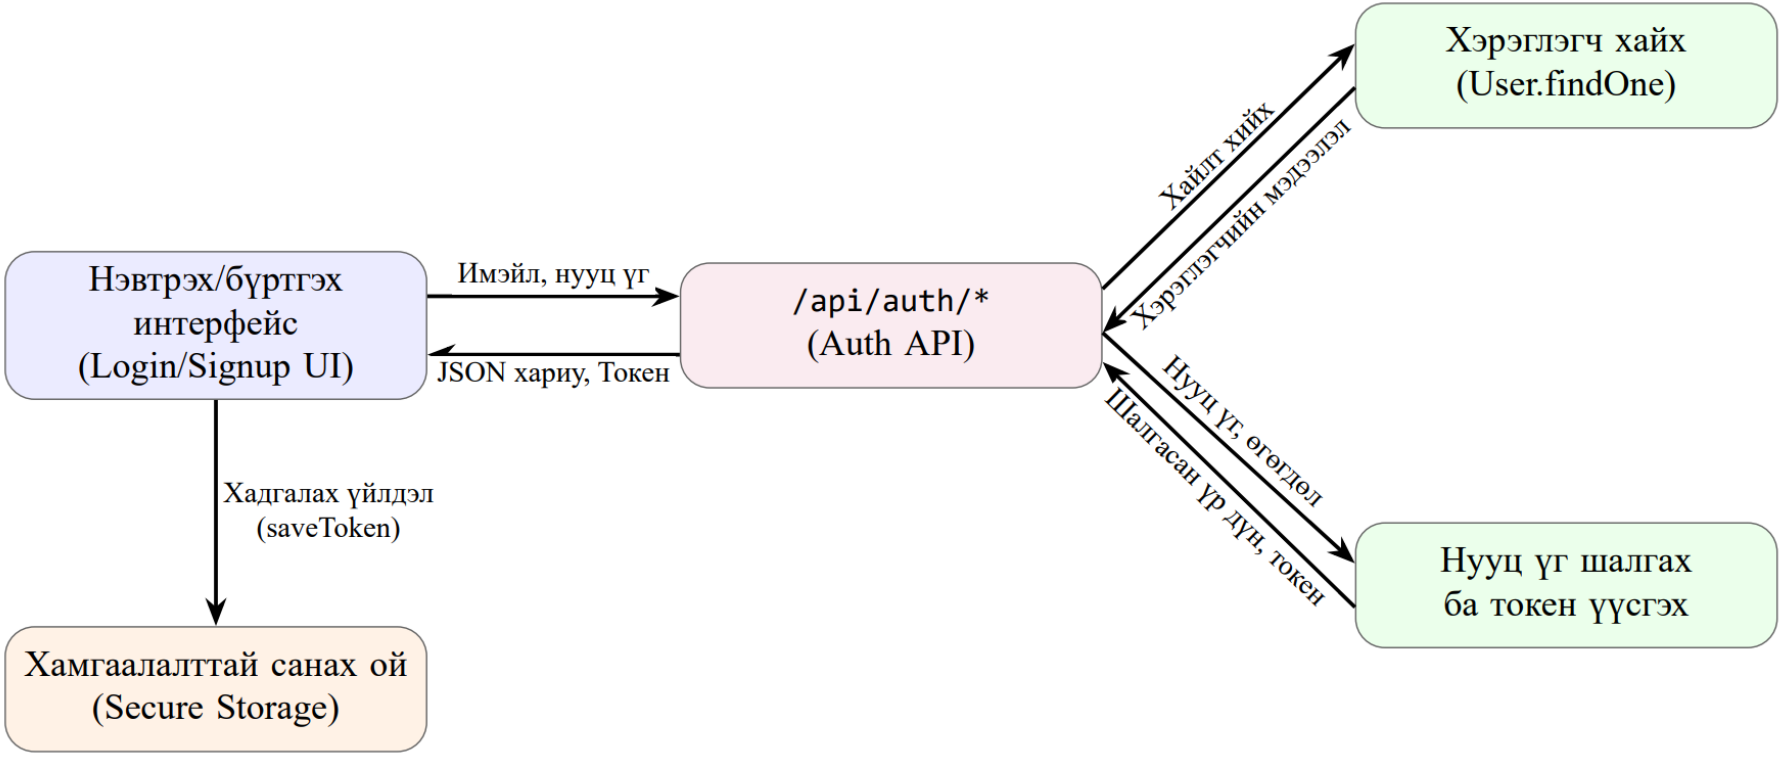
\includegraphics[width=0.95\textwidth]{Pictures/3,4.png}
\caption{Хоёрдугаар түвшний өгөгдлийн урсгал: нэвтрэх болон бүртгэх урсгал}
\label{fig:dfd_auth_detail}
\end{figure}

\noindent \fref{fig:dfd_auth_detail}-д хэрэглэгчийн бүртгэл/нэвтрэлтийн хүсэлт серверт дамжиж, хэрэглэгчийн мэдээлэл шалгах, нууц үг баталгаажуулах, JWT токен үүсгэх, токентой хариу буцаах дарааллыг өгөгдлийн урсгалын түвшинд дэлгэрүүлэн үзүүлэв.

\subsection{Тэмдэглэлийн CRUD урсгалын өгөгдлийн зураг}

\begin{figure}[H]
\centering
\makebox[\textwidth][c]{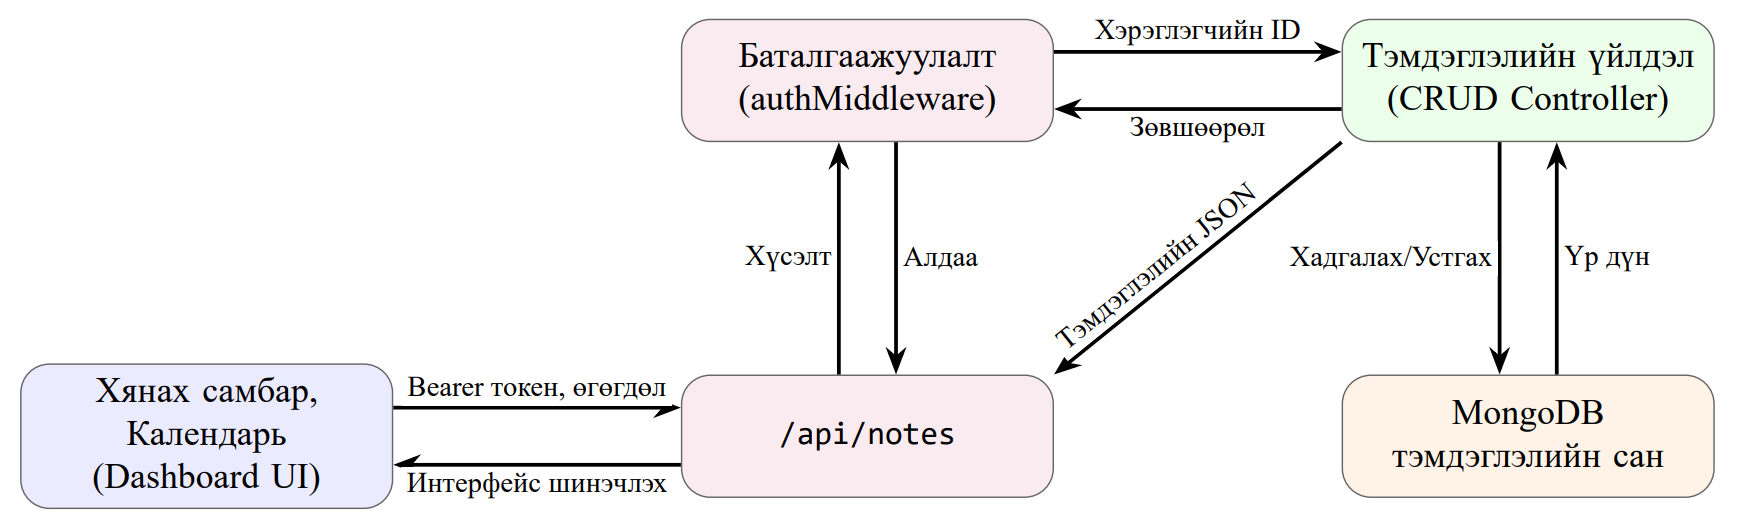
\includegraphics[width=0.98\textwidth]{Pictures/2r_tuvshin_3.png}}
\caption{Хоёрдугаар түвшний өгөгдлийн урсгал: тэмдэглэлийн CRUD урсгал}
\label{fig:dfd_notes_detail}
\end{figure}

\noindent \fref{fig:dfd_notes_detail}-д хэрэглэгчийн тэмдэглэлтэй холбоотой CRUD үйлдлийн өгөгдлийн урсгалыг харуулсан. Хэрэглэгчийн интерфейсээс илгээсэн хүсэлт \texttt{/api/notes} endpoint-оор дамжин эхлээд баталгаажуулалтын завсрын модульд (authentication middleware) шалгагдаж, зөвшөөрөгдсөн тохиолдолд хянагч модуль (controller) руу шилжин MongoDB мэдээллийн санд хадгалах, унших, шинэчлэх, устгах үйлдлүүдийг гүйцэтгэнэ.

\subsection{Стикер үүсгэх урсгалын өгөгдлийн зураг}

\begin{figure}[H]
\centering
\makebox[\textwidth][c]{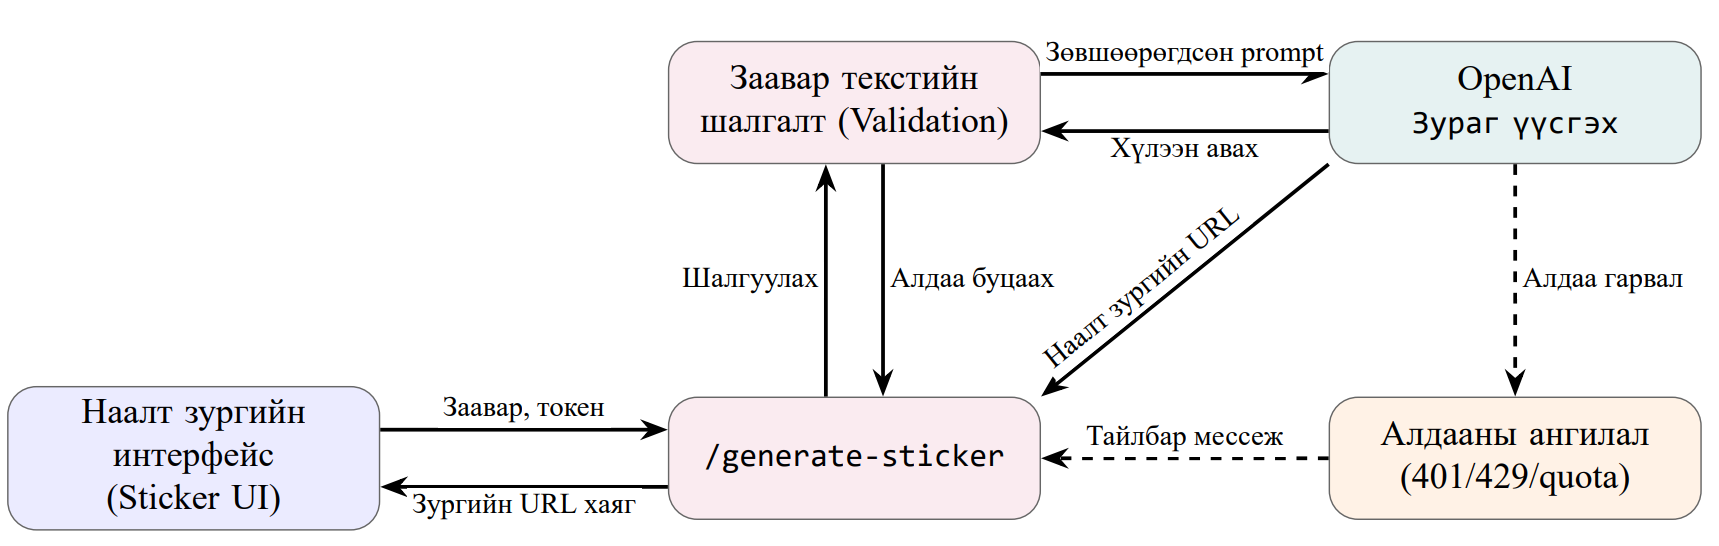
\includegraphics[width=0.98\textwidth]{Pictures/2r_tuvshin4.png}}
\caption{Хоёрдугаар түвшний өгөгдлийн урсгал: хиймэл оюун ухаанаар стикер үүсгэх урсгал (AI sticker generation)}
\label{fig:dfd_sticker_detail}
\end{figure}

\noindent \fref{fig:dfd_sticker_detail}-д хиймэл оюунд суурилсан стикер үүсгэх урсгалыг үзүүлсэн. Хэрэглэгчийн хүсэлт \texttt{/api/notes/generate-sticker} endpoint-оор орж, заавар текстийн шалгалтаар (validation) баталгаажсаны дараа OpenRouter API руу дамжуулан зураг үүсгэж, стикерийн холбоосыг клиент талд буцаах замналаар загварчлав.

\subsection{Өгөгдлийн урсгалын диаграммын тайлбар ба нэгтгэл}

Өгөгдлийн урсгалын диаграмм (DFD)-ыг энэ судалгаанд системийн логикийг шаталсан түвшинд ойлгомжтой тайлбарлах зорилгоор ашигласан. Диаграммын үндсэн тэмдэглэгээг дараах байдлаар хэрэглэв:

\begin{itemize}
    \item \textbf{Гаднах оролцогч (External entity):} системээс гадуурх хэрэглэгч эсвэл үйлчилгээ;
    \item \textbf{Процесс (Process):} өгөгдөл боловсруулж дараагийн шат руу шилжүүлдэг дотоод модуль;
    \item \textbf{Өгөгдлийн сан (Data store):} тогтмол хадгалалт хийгдэх мэдээллийн цэг;
    \item \textbf{Өгөгдлийн урсгал (Data flow):} модулиудын хооронд дамжих хүсэлт, хариу, бизнес өгөгдөл.
\end{itemize}

\begin{table}[H]
\centering
\caption{Өгөгдлийн урсгалын диаграммын түвшинчилсэн тайлбарын нэгтгэл}
\label{tab:dfd_explanation_summary}
\small
\setlength{\tabcolsep}{4pt}
\renewcommand{\arraystretch}{1.15}
\begin{tabularx}{\textwidth}{>{\raggedright\arraybackslash}p{2.2cm}>{\raggedright\arraybackslash}p{3.2cm}>{\raggedright\arraybackslash}X>{\raggedright\arraybackslash}p{2.4cm}}
\toprule
\textbf{Түвшин} & \textbf{Гол урсгал} & \textbf{Тайлбар} & \textbf{Зорилго} \\
\midrule
Контекст (Зураг 4.2) & Систем ба гадаад орчин & Хэрэглэгчийн UI хүсэлт системд орж, систем MongoDB болон OpenRouter API-тай өгөгдөл солилцох ерөнхий урсгалыг харуулсан. & Системийн хил хязгаар тодорхойлох \\
Нэгдүгээр түвшин (Зураг 4.3) & P1 Auth, P2 Notes, P3 Sticker & Контекст түвшний нэг процессыг баталгаажуулалт, тэмдэглэлийн CRUD, AI стикерийн модулиудад задалж, өгөгдлийн сан/гадаад үйлчилгээтэй харилцах логикийг харуулсан. & Архитектурын модульчилсан задаргаа \\
Хоёрдугаар түвшин (Зураг 4.4) & Нэвтрэх/бүртгэх урсгал & Хэрэглэгчийн бүртгэл, нэвтрэлт, нууц үгийн шалгалт, JWT токен үүсэлт ба хариу өгөгдлийн урсгалыг дэлгэрүүлсэн. & Auth урсгал баталгаажуулах \\
Хоёрдугаар түвшин (Зураг 4.5--4.6) & CRUD, Sticker урсгал & Тэмдэглэлийн CRUD болон AI стикер үүсгэх урсгалыг endpoint түвшинд нарийвчлан үзүүлсэн. & Гол бизнес урсгал баталгаажуулах \\
\bottomrule
\end{tabularx}
\normalsize
\end{table}

Ийнхүү DFD-ийг контекстээс нарийвчилсан түвшин рүү буулгаснаар системийн өгөгдөл дамжих дараалал, хариуцлагын зааг, баталгаажуулалтын цэгүүдийг судалгааны бичвэрт нотолгоотойгоор тайлбарлах боломж бүрдсэн.

\section{Дарааллын диаграммууд (sequence diagrams)}

Өгөгдлийн урсгалын зураг (dataflow) нь өгөгдөл хаашаа урсаж байгааг харуулдаг бол дарааллын диаграмм (sequence diagram) нь \textbf{цаг хугацааны дараалал}-ыг тодорхой харуулдаг. Энэ ажлын үндсэн гурван урсгалд дарааллын диаграмм (sequence diagram) ашиглав.

\subsection{Дарааллын диаграмм 1: Нэвтрэх урсгал}

\begin{figure}[H]
\centering
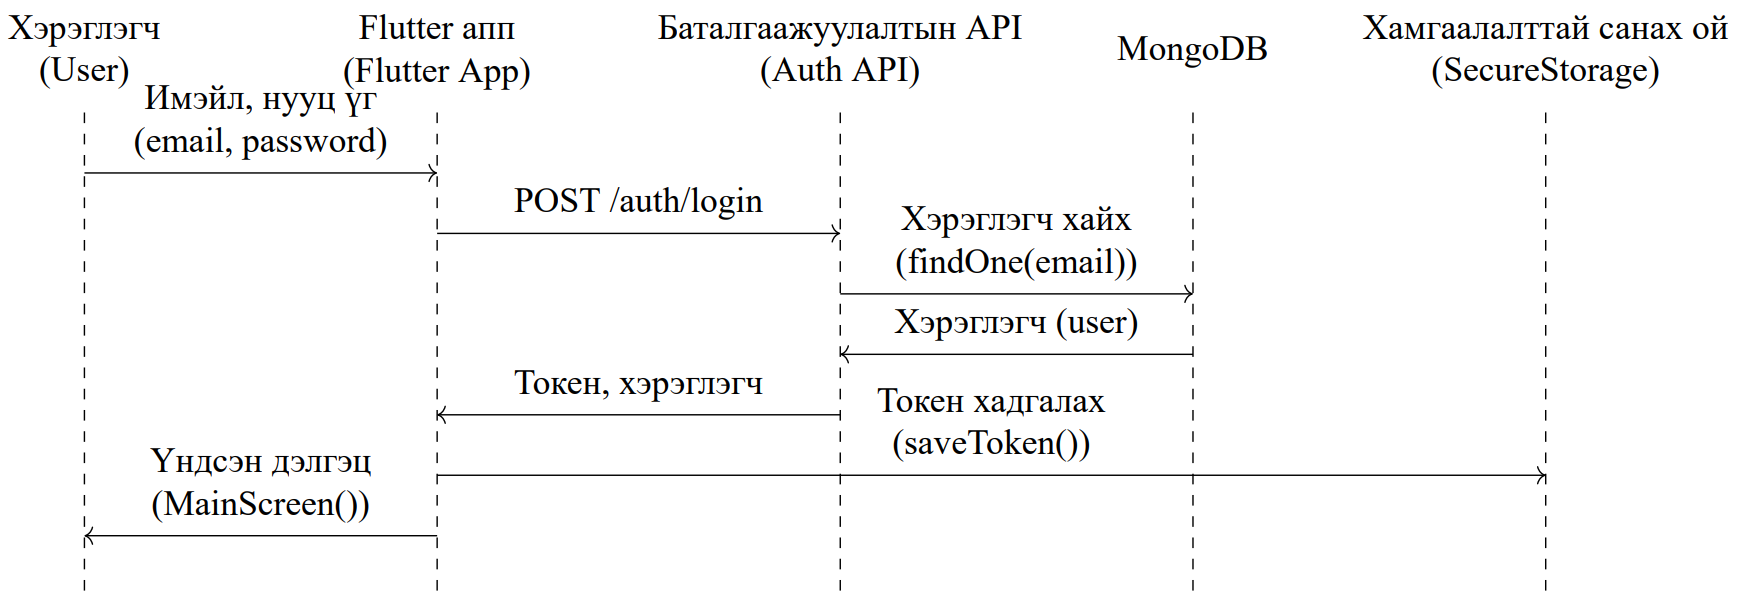
\includegraphics[width=0.95\textwidth]{Pictures/nevtreh1.png}
\caption{Дарааллын диаграмм: нэвтрэх урсгал}
\label{fig:seq_login}
\end{figure}

\noindent \fref{fig:seq_login}-д хэрэглэгч нэвтрэх мэдээллээ илгээснээс эхлэн сервер талд хэрэглэгч шалгах, нууц үг баталгаажуулах, JWT токен үүсгэх, улмаар апп талд токен хадгалж үндсэн дэлгэц рүү шилжих хүртэлх хугацааны дарааллыг харуулсан.

\subsection{Дарааллын диаграмм 2: Тэмдэглэл үүсгэх урсгал}

\begin{figure}[H]
\centering
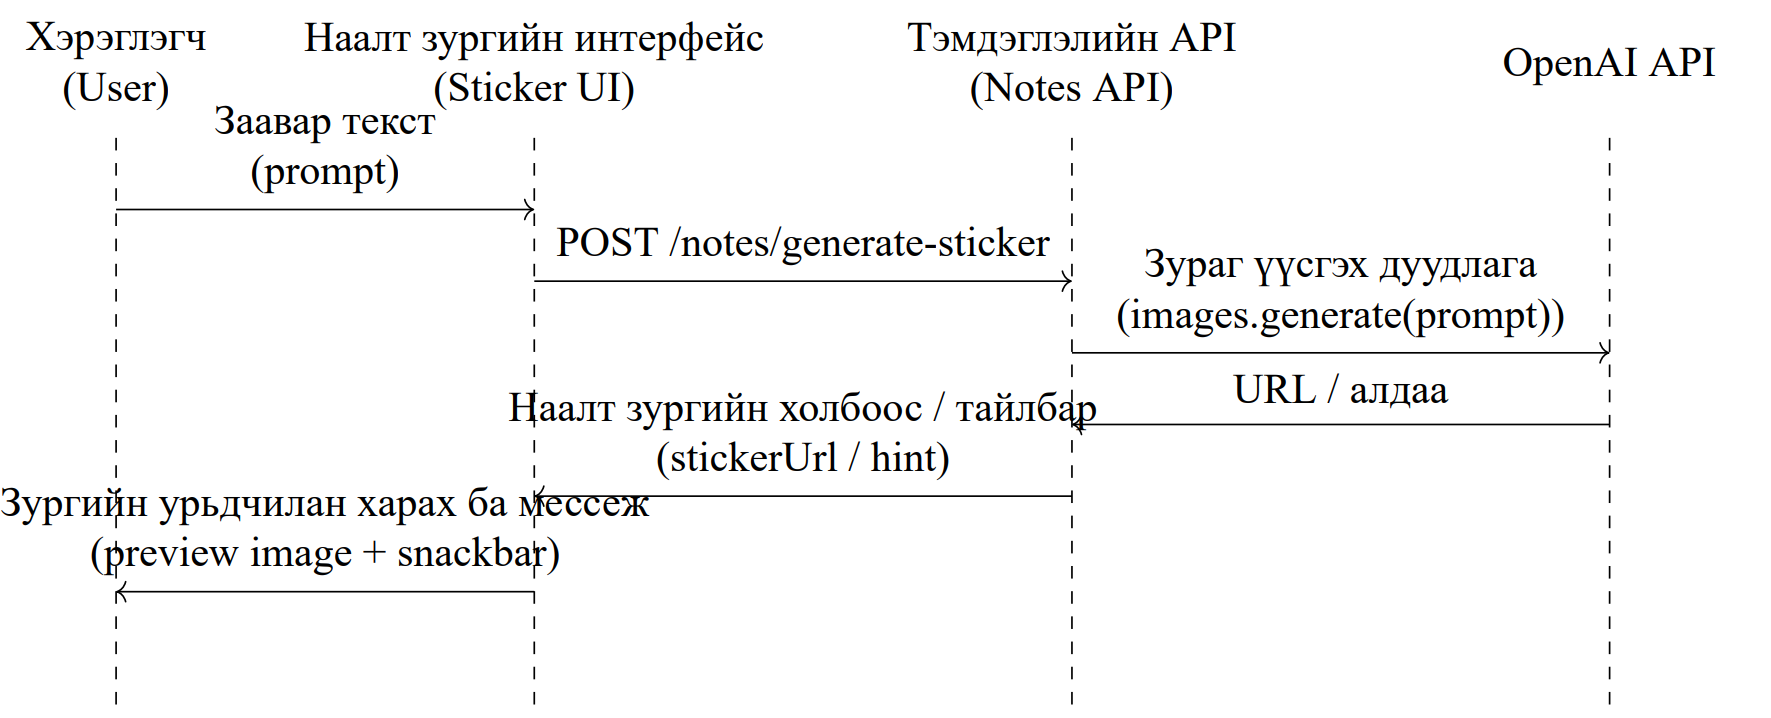
\includegraphics[width=0.95\textwidth]{Pictures/nevtreh3.png}
\caption{Дарааллын диаграмм: тэмдэглэл үүсгэх урсгал}
\label{fig:seq_note_create}
\end{figure}

\noindent \fref{fig:seq_note_create}-д шинэ тэмдэглэл үүсгэх хүсэлт токеноор баталгаажсаны дараа серверт хадгалагдаж, хариу өгөгдөл клиент талд ирэхэд жагсаалт болон интерфейсийн төлөв шинэчлэгдэх үе шат бүрийг дарааллаар нь үзүүлэв.

\subsection{Дарааллын диаграмм 3: Хиймэл оюун ухаанаар стикер үүсгэх урсгал (AI sticker generation)}

\begin{figure}[H]
\centering
\begin{tikzpicture}[
    font=\small,
    every node/.style={align=center},
    lbl/.style={fill=white, inner sep=1.2pt, font=\scriptsize}
]
\node at (0,0) {Хэрэглэгч\\(User)};
\node at (4,0) {стикерийн интерфейс\\(Sticker UI)};
\node at (8,0) {Тэмдэглэлийн API\\(Notes API)};
\node at (12,0) {OpenRouter API};

\foreach \x in {0,4,8,12} {\draw[dashed] (\x,-0.4) -- (\x,-6.0);} 

\draw[->] (0,-1.1) -- node[above, lbl] {Заавар текст\\(prompt)} (4,-1.1);
\draw[->] (4,-1.9) -- node[above, lbl] {POST /notes\\generate-sticker} (8,-1.9);
\draw[->] (8,-2.7) -- node[above, lbl] {Зураг үүсгэх\\дуудлага\\images.generate(prompt)} (12,-2.7);
\draw[->] (12,-3.5) -- node[above, lbl] {URL / алдаа} (8,-3.5);
\draw[->] (8,-4.3) -- node[above, lbl] {стикерийн холбоос\\(stickerUrl / hint)} (4,-4.3);
\draw[->] (4,-5.1) -- node[above, lbl] {Урьдчилан харах ба мессеж\\(preview + snackbar)} (0,-5.1);
\end{tikzpicture}
\caption{Дарааллын диаграмм: хиймэл оюун ухаанаар стикер үүсгэх урсгал (AI sticker generation)}
\label{fig:seq_sticker}
\end{figure}

\noindent \fref{fig:seq_sticker}-д заавар текст (prompt) клиентээс сервер рүү дамжин OpenRouter API үйлчилгээ дуудсаны дараа стикерийн URL эсвэл алдааны мэдээлэл буцаж, хэрэглэгчид урьдчилан харах болон мессеж хэлбэрээр хүрэх логикийг хугацааны тэнхлэгээр дүрсэлсэн.

\section{Хэрэглээний тохиолдлын загвар (Use Case Diagram)}

Хэрэглээний тохиолдлын диаграмм (use case diagram) нь системийн функционал хил хязгаар (system boundary) болон хэрэглэгчийн оролцооны үүргийг ерөнхий түвшинд тодорхойлох зорилготой. Энэ нь өгөгдлийн урсгал (dataflow) ба дарааллын диаграмм (sequence diagram)-ын өмнөх ойлголтын гүүр болж, хэрэглэгч системтэй яг ямар зорилгоор харилцаж байгааг нэг зурагт нэгтгэн харуулдаг.

Энэхүү судалгаанд үндсэн оролцогчоор эцсийн хэрэглэгч (mobile user)-ийг авч үзэж, нэвтрэх/бүртгэх, тэмдэглэл удирдах, календарь харах, стикер үүсгэх, сануулга-мэдэгдэлтэй ажиллах гэсэн гол хэрэглээний тохиолдлуудыг загварчилсан.

\begin{figure}[H]
\centering
\resizebox{0.9\textwidth}{!}{%
\begin{tikzpicture}[
    font=\small,
    uc/.style={ellipse, draw=purple!70, fill=purple!8, minimum width=8.1cm, minimum height=1.1cm, align=center},
    actorlbl/.style={font=\small}
]

% Actor (stick figure)
\coordinate (ah) at (-7.8,2.2);
\draw[thick] (ah) circle (0.35);
\draw[thick] (-7.8,1.85) -- (-7.8,0.75);
\draw[thick] (-8.4,1.4) -- (-7.2,1.4);
\draw[thick] (-7.8,0.75) -- (-8.25,-0.2);
\draw[thick] (-7.8,0.75) -- (-7.35,-0.2);
\node[actorlbl] at (-7.8,-0.6) {Хэрэглэгч};

% System boundary
\draw[rounded corners=10pt, thick, draw=blue!60] (-5.4,-4.0) rectangle (8.8,4.0);
\node[anchor=north west, font=\bfseries\small] at (-5.2,3.8) {AI Notebook систем};

% Use cases
\node[uc] (ucAuth) at (1.7,2.9) {Бүртгэх / Нэвтрэх};
\node[uc] (ucNotes) at (1.7,1.4) {Тэмдэглэл үүсгэх, засах, устгах};
\node[uc] (ucCalendar) at (1.7,-0.1) {Календарь дээрээс тэмдэглэл харах};
\node[uc] (ucSticker) at (1.7,-1.6) {Хиймэл оюун ухаанаар стикер үүсгэх};
\node[uc] (ucNotif) at (1.7,-3.1) {Сануулга тохируулах, мэдэгдэл харах};

% Associations
\draw[thick] (-7.2,1.4) -- (ucAuth.west);
\draw[thick] (-7.2,1.4) -- (ucNotes.west);
\draw[thick] (-7.2,1.4) -- (ucCalendar.west);
\draw[thick] (-7.2,1.4) -- (ucSticker.west);
\draw[thick] (-7.2,1.4) -- (ucNotif.west);

\end{tikzpicture}%
}
\caption{AI Notebook системийн хэрэглээний тохиолдлын диаграмм}
\label{fig:usecase_overview}
\end{figure}

\section{Өгөгдлийн сангийн ER диаграмм (Entity-Relationship Diagram)}

Энэ хэсэгт AI Notebook системийн өгөгдлийн бүтэц болон entity хоорондын хамаарлыг харуулав. Үндсэн тэмдэглэгээний хэлбэр нь \texttt{||-->} бөгөөд энд \texttt{||} = яг нэг (mandatory one), \texttt{>} = олон (many) гэсэн утгатай.

\begin{figure}[H]
\centering
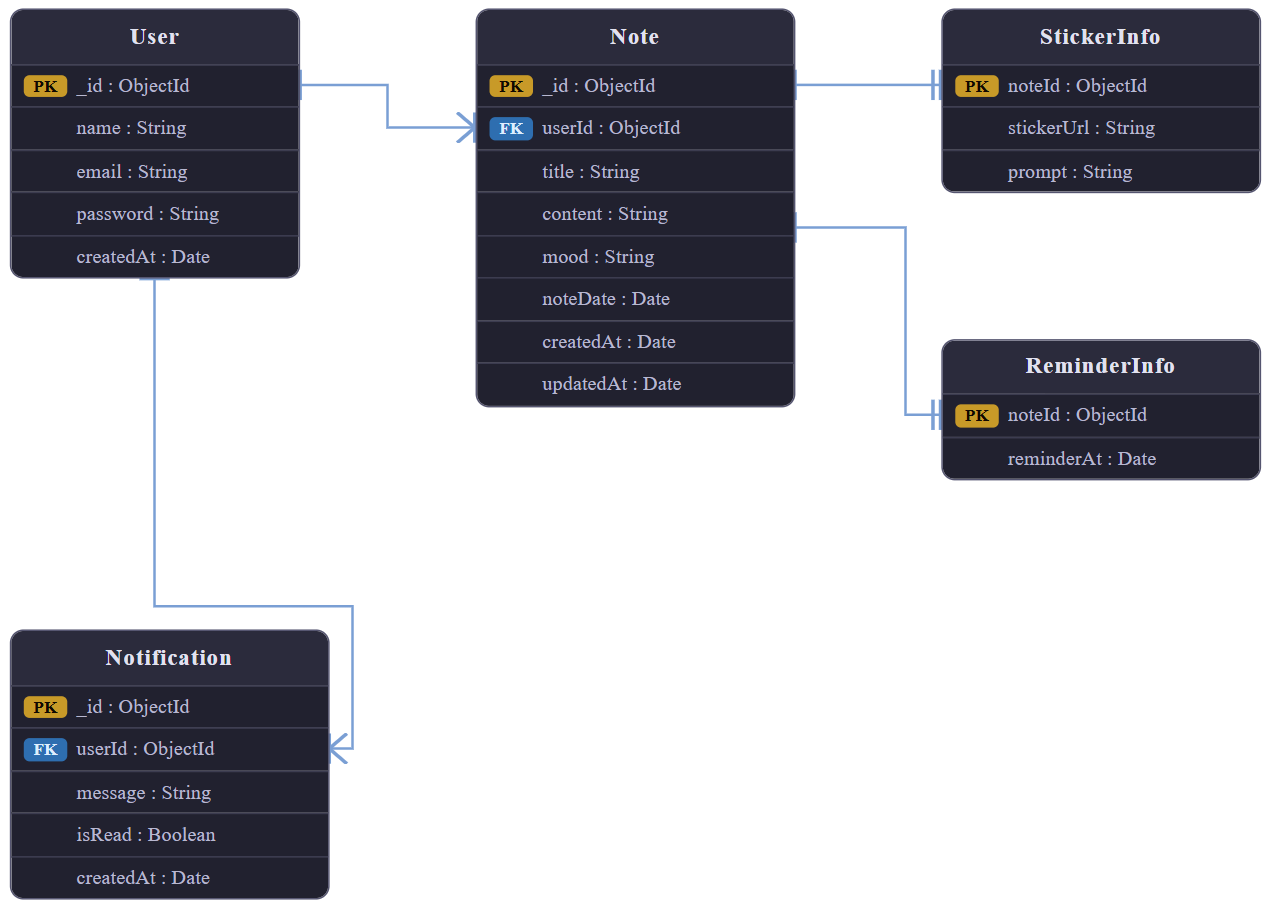
\includegraphics[width=0.98\textwidth]{Pictures/ERD.png}
\caption{AI Notebook системийн өгөгдлийн сангийн ER диаграммын задаргаа}
\label{fig:erd_overview}
\end{figure}

\noindent \fref{fig:erd_overview}-ийн харилцааны утга нь дараах байдалтай.

\begin{itemize}
    \item \texttt{User ||-> Note}: нэг хэрэглэгч олон тэмдэглэлтэй.
    \item \texttt{Note ||--|| StickerInfo}: нэг тэмдэглэлд нэг стикерийн мэдээлэл холбогдоно (логикийн хувьд \texttt{0..1} буюу optional).
    \item \texttt{Note ||--|| ReminderInfo}: нэг тэмдэглэлд нэг сануулгын мэдээлэл холбогдоно (логикийн хувьд \texttt{0..1} буюу optional).
    \item \texttt{User ||-> Notification}: нэг хэрэглэгч олон мэдэгдэл хүлээн авна.
\end{itemize}

\noindent PK/FK-ийн товч тайлбар:

\begin{itemize}
    \item \textbf{PK (Primary Key)}: хүснэгтийн мөр бүрийг давтагдашгүй таних үндсэн түлхүүр. Жишээ нь \texttt{User.\_id}, \texttt{Note.\_id}.
    \item \textbf{FK (Foreign Key)}: өөр entity-ийн PK-руу заасан холбоос түлхүүр. Жишээ нь \texttt{Note.userId $\rightarrow$ User.\_id}. Энэ холбоосоор тэмдэглэл аль хэрэглэгчтэй хамаарахыг тогтооно.
\end{itemize}

\noindent Тайлбар: концепцийн ERD дээр \texttt{StickerInfo} ба \texttt{ReminderInfo}-г тусдаа entity хэлбэрээр үзүүлсэн. Харин бодит MongoDB хэрэгжилтэд эдгээр нь \texttt{Note} document доторх \texttt{stickerUrl} болон \texttt{reminderAt} nullable талбаруудаар хадгалагдана.

\section{Шалгуур}

Системийн урсгал бүрийг дараах шалгуураар баталгаажуулсан:

\begin{itemize}
    \item Баталгаажуулалтын урсгал (auth flow): токен олголт, хадгалалт, дэлгэц шилжилтийн (navigation) зөв байдал;
    \item Тэмдэглэлийн урсгал (notes flow): CRUD үйлдлийн дараах өгөгдлийн тууштай байдал;
    \item стикерийн урсгал (sticker flow): заавар текстээс (prompt) URL буцах, алдааны тайлбар зөв харуулах эсэх;
    \item Мэдэгдлийн урсгал (notification flow): сануулгыг зөв хуваарьлах/цуцлах, мэдэгдлийн жагсаалтын төлөв шинэчлэх;
    \item Аюулгүй байдлын урсгал (security flow): токенгүй хүсэлтэд 401 буцах эсэх.
\end{itemize}

\section{Generative AI туршилтын аргачлал}

Энэхүү судалгаанд хиймэл оюун ухаанд суурилсан \texttt{/api/notes/generate-sticker} төгсгөлийн цэгийг (endpoint) бодит орчинд шалгаж, үр дүнг зөвхөн дараах хоёр метрикаар үнэлэв.

\begin{enumerate}
    \item \textbf{Latency} (зураг үүсгэх хугацаа, секунд),
    \item \textbf{Prompt relevance} (үсгэсэн зураг prompt-той нийцэж байгаа эсэх).
\end{enumerate}

Туршилтыг 2026-04-17-нд Windows орчинд ажилласан Node.js backend дээр хийж, баталгаажуулалтын (JWT) токентой хүсэлтүүдийг \texttt{Invoke-RestMethod} ашиглан давтан илгээсэн.

\subsection*{Latency хэмжих арга}

Хүсэлт бүрийн эхлэх ба дуусах хугацааг тэмдэглэж, зураг үүсгэх хугацааг секундээр тооцов:
\begin{equation}
\label{eq:latency}
t_{\mathrm{latency}} = t_{\mathrm{response}} - t_{\mathrm{request}}\; (\mathrm{sec})
\end{equation}

Нэг сценар доторх дундаж хугацааг:
\begin{equation}
\label{eq:mean_latency}
\overline{t} = \frac{1}{N}\sum_{i=1}^{N} t_i
\end{equation}
томьёогоор гаргав.

\subsection*{Generative AI туршилтын сценарийн дефиниц}

Generative AI гүйцэтгэлийг үнэлэхийн тулд OpenRouter fallback стратегийн өөр өөр сценарийг туршив:

\begin{itemize}
    \item \textbf{S1 (Internal fallback, unique prompt)}: Уникаль prompt бүрэлмж ашиглаж, гаднын OpenRouter үйлчилгээ суугдахгүйгээр дотоод fallback (cached sticker templates) ашигласан. $N=40$ давтуулгаар дотоод механизмын үр ашиг, CPU ачаалалыг хэмжив. Хүлээгдсэн үр дүн: хамгийн бага latency, тогтвортой performance.
    
    \item \textbf{S2 (Designed fallback, unique prompt, network latency)}: Уникаль prompt-ыг OpenRouter рүү дамжүүлэх үед сүлжээний саатлыг симуляцлаж ($N=10$ давтуулга), OpenRouter амжилтгүй болох үед system дотоод fallback руу шилжихийн үр дүнг хэмжив. Энэ сценарт ambiguous/complex prompt-уудыг ашигласан. Хүлээгдсэн үр дүн: өндөр latency variation, fallback source-ийн сонголт, дараа дахь retry стратегийн үр нөлөө.
    
    \item \textbf{S3 (Designed fallback, cached prompt)}: Өмнө үүсгэн хадгалсан prompt-ыг давтан ашиглаж ($N=10$ давтуулга), кэшэ дэх өмнөх үр дүнг ашигласан. Хүлээгдсэн үр дүн: хамгийн бага latency, 100\% hit rate, caching механизмын үр ашиг.
\end{itemize}

\subsection*{Prompt relevance үнэлэх арга}

 Үүсгэсэн зураг бүрийг prompt-ийн үндсэн утгатай тохирч байгаа эсэхээр бинар үнэлэв:

\begin{itemize}
    \item \textbf{1 (нийцсэн)}: prompt-д өгсөн гол объект/үйлдэл зурагт тодорхой харагдсан,
    \item \textbf{0 (нийцээгүй)}: prompt-ийн гол утга алдагдсан эсвэл өөр сэдэв рүү хазайсан.
\end{itemize}

Нийцлийн хувийг дараах байдлаар тооцов:
\begin{equation}
\label{eq:prompt_relevance}
\text{Prompt relevance rate}(\%) = \frac{N_{\mathrm{match}}}{N_{\mathrm{total}}} \times 100
\end{equation}
энд $N_{match}$ нь нийцсэн зураг, $N_{total}$ нь нийт үүсгэсэн зураг болно.

\section{Туршилтын протокол ба өгөгдөл цуглуулах зохион байгуулалт}

Энэхүү судалгаанд туршилтыг "бэлтгэл -- гүйцэтгэл -- баталгаажуулалт -- бүртгэл" гэсэн дөрвөн үе шаттай протоколоор хийсэн. Протоколчилсон шалтгаан нь туршилтын давтагдахуйц чанарыг (reproducibility) нэмэгдүүлж, хэмжилтийн ялгааг орчны санамсаргүй нөлөөнөөс тусгаарлах явдал юм.

\begin{enumerate}
    \item \textbf{Бэлтгэл:} backend орчны хувьсагч (JWT, database, OpenRouter key), тест хэрэглэгч, үндсэн датаг ижил нөхцөлөөр бэлдэх;
    \item \textbf{Гүйцэтгэл:} сценар тус бүрт ижил payload, ижил endpoint дараалал ашиглах;
    \item \textbf{Баталгаажуулалт:} HTTP статус, response body, UI төлөв, өгөгдлийн сангийн үр дүнг зэрэг шалгах;
    \item \textbf{Бүртгэл:} latency, алдаа, fallback эх үүсвэр, CPU ажиглалтыг нэг загвараар тэмдэглэх.
\end{enumerate}

\begin{table}[H]
\centering
\caption{Туршилтын протоколын нэгтгэл}
\label{tab:test_protocol_summary}
\small
\setlength{\tabcolsep}{4pt}
\renewcommand{\arraystretch}{1.15}
\begin{tabularx}{\textwidth}{>{\raggedright\arraybackslash}p{2.0cm}>{\raggedright\arraybackslash}X>{\raggedright\arraybackslash}p{3.0cm}>{\raggedright\arraybackslash}p{2.4cm}}
\toprule
\textbf{Сценар} & \textbf{Товч тодорхойлолт} & \textbf{Гол хэмжилт} & \textbf{Хүлээгдсэн үр дүн} \\
\midrule
AUTH-01 & Зөв credential-ээр нэвтрэх & HTTP 200, token field & Амжилттай нэвтрэлт \\
AUTH-02 & Токенгүй хамгаалалттай endpoint дуудах & HTTP 401 & Хандалт хориглогдох \\
CRUD-01 & Тэмдэглэл үүсгэх/засах/устгах дараалал & DB change + UI refresh & Өгөгдлийн тууштай байдал \\
AI-01 & Уникаль prompt-оор стикер үүсгэх & Latency, response source & URL эсвэл fallback хариу \\
AI-02 & Давтагдсан prompt урсгал & Latency variation, cache/fallback behavior & Тогтвортой response хэв шинж \\
NOTIF-01 & Reminder тохируулах ба хүргэх & Trigger time, notification event & Хугацаанд нийцсэн мэдэгдэл \\
\bottomrule
\end{tabularx}
\normalsize
\end{table}

Өгөгдөл цуглуулахдаа хэмжилтийн бүртгэлийг нэг форматаар хадгалж, алдааны тохиолдолд endpoint, payload төрөл, хариу код, fallback эх үүсвэрийг тусад нь тэмдэглэсэн. Ийнхүү структурчилсан бүртгэл нь үр дүнг дараа нь бүлэглэж шинжлэх, орчны шалтгаант хэлбэлзлийг тайлбарлах боломжийг нэмэгдүүлсэн.

\section{Хүчин төгөлдөр байдлын эрсдэл ба бууруулах арга}

Судалгааны арга зүйн найдвартай байдлыг үнэлэхдээ дотоод (internal), гадаад (external), бүтэц-ойлголтын (construct) болон дүгнэлтийн (conclusion) хүчин төгөлдөр байдлын эрсдлийг ялган авч үзэв.

\begin{table}[H]
\centering
\caption{Хүчин төгөлдөр байдлын эрсдэл ба бууруулах стратеги}
\label{tab:validity_threats}
\small
\setlength{\tabcolsep}{4pt}
\renewcommand{\arraystretch}{1.15}
\begin{tabularx}{\textwidth}{>{\raggedright\arraybackslash}p{2.8cm}>{\raggedright\arraybackslash}X>{\raggedright\arraybackslash}p{3.9cm}}
\toprule
\textbf{Эрсдэлийн төрөл} & \textbf{Болзошгүй нөлөө} & \textbf{Бууруулах арга} \\
\midrule
Дотоод хүчин төгөлдөр байдал & Орчны тохиргоо өөрчлөгдвөл тестийн үр дүн зөрөх & Нэг орчинд ижил протоколоор давтан гүйцэтгэл хийх \\
Гадаад хүчин төгөлдөр байдал & Нэг хэрэглэгч/нэг төхөөрөмжийн дүн бүх хэрэглээнд шууд ерөнхийшөхгүй байх & Өөр сценар, өөр prompt багц ашиглан харьцуулсан үнэлгээ хийх \\
Construct validity & "Чанар" ойлголтыг буруу метрикаар төлөөлөх эрсдэл & Latency, статус код, UX feedback зэрэг олон индикатор хослуулах \\
Conclusion validity & Бага хэмжээний сорьц дээр хэт ерөнхий дүгнэлт хийх эрсдэл & p50/p95, mean, max зэрэг тархалтын үзүүлэлтээр тайлбарлах \\
\bottomrule
\end{tabularx}
\normalsize
\end{table}

Ийм эрсдэлийн шинжилгээг арга зүйн хэсэгт тусгаснаар судалгааны үр дүн нь зөвхөн эерэг кейсийн тайлбар бус, баталгаажуулалтын хязгаарлалтаа ил тод тэмдэглэсэн академик бүтцэд шилжиж байна.



% 5-р бүлэг: Судалгааны үр дүн, дүгнэлт
\chapter{Судалгааны үр дүн}
\label{ch:results}

\section{Хэрэгжилтийн үр дүнгийн тойм}

Энэхүү судалгааны хүрээнд AI Notebook системийн харагдах хэсэг (frontend), сервер талын хэсэг (backend), өгөгдлийн сан, хиймэл оюуны интеграц гэсэн үндсэн бүрэлдэхүүнүүд бүрэн хэрэгжиж, хоорондын уялдаа ажиллах түвшинд хүрсэн. Үр дүнг системийн түвшинд авч үзвэл:

\begin{enumerate}
    \item Хэрэглэгчийн баталгаажуулалтын урсгал амжилттай,
    \item Тэмдэглэлийн амьдралын мөчлөг (note lifecycle: үүсгэх-засах-устгах) тогтвортой,
    \item Календарь болон сэтгэл хөдлөлийн төлөвөөр (mood) тэмдэглэл харах боломж хэрэгжсэн,
    \item Хиймэл оюун ухаанаар стикер үүсгэх (AI sticker generation) төгсгөлийн цэг амжилттай интеграцчлагдсан,
    \item JWT завсрын модуль (middleware)-аар хамгаалагдсан API зохих ёсоор ажилласан.
\end{enumerate}

\section{Өгөгдлийн урсгалын зурагт суурилсан баталгаажуулалт (dataflow)}

Арга зүйн бүлэгт тодорхойлсон \fref{fig:dfd_context}, \fref{fig:dfd_level1}, \fref{fig:dfd_auth_detail}, \fref{fig:dfd_notes_detail}, \fref{fig:dfd_sticker_detail} диаграммууд дээрх урсгал бүрийг бодит кодын зан төлөвтэй харьцуулан шалгав.

\begin{table}[H]
\centering
\caption{Өгөгдлийн урсгалын түвшний баталгаажуулалтын нэгтгэл}
\label{tab:dataflow_validation}
\begin{tabular}{>{\raggedright\arraybackslash}p{3.8cm}>{\raggedright\arraybackslash}p{6.5cm}>{\raggedright\arraybackslash}p{2.8cm}}
\toprule
\textbf{Урсгал} & \textbf{Баталгаажсан шалгалт} & \textbf{Дүн} \\
\midrule
Баталгаажуулалтын урсгал (Auth flow) & /api/auth/login, /api/auth/signup урсгалд токен болон хэрэглэгчийн мэдээлэл буцаж, хамгаалалттай санах ойд (Secure Storage) хадгалагдсан & Амжилттай \\
Тэмдэглэлийн урсгал (Notes flow) & /api/notes төрлийн CRUD хүсэлт бүр завсрын модуль (middleware)-ээр дамжин зөвхөн тухайн хэрэглэгчийн өгөгдөлд үйлчилсэн & Амжилттай \\
Наалт зургийн урсгал (Sticker flow) & /api/notes/generate-sticker урсгал заавар текст (prompt) авч OpenAI руу дамжуулан наалт зургийн URL буцаасан & Амжилттай \\
Алдааны урсгал (Error flow) & API түлхүүр (key), хязгаарлалт (quota), сүлжээний (network) алдааг харагдах хэсэгт (frontend) тайлбартай мессеж (snackbar) болгон харуулсан & Амжилттай \\
\bottomrule
\end{tabular}
\end{table}

\section{Дарааллын диаграммын түвшний баталгаажуулалт (sequence)}

\fref{fig:seq_login}, \fref{fig:seq_note_create}, \fref{fig:seq_sticker} гэсэн дарааллын (sequence) диаграммуудаар харуулсан хугацааны дарааллыг туршилтаар дараах байдлаар баталгаажуулав.

\begin{enumerate}
    \item Нэвтрэх (login) үед хэрэглэгч шалгах, нууц үгийг баталгаажуулах, токен үүсгэх дараалал хэвийн ажилласан. Үүний дараа дотоод хадгалалт шинэчлэгдсэн.
    \item Тэмдэглэл үүсгэх (note create) үед токен баталгаажуулах, хэрэглэгчийн эрхийг тогтоох, өгөгдөл хадгалах, интерфейс шинэчлэх дараалал тасалдаагүй.
    \item Наалт зураг үүсгэх (sticker generate) үед заавар текст (prompt) шалгах, AI үйлчилгээ рүү дамжуулах, URL хариу буцаах дараалал тогтвортой ажилласан.
\end{enumerate}

\section{Харагдах хэсгийн (frontend) хөгжүүлэлтийн үр дүн}

Flutter дээрх харагдах хэсэгт (frontend) дараах үндсэн дэлгэцүүдийг бүтээсэн:

\begin{itemize}
    \item Нэвтрэх/бүртгэх (Login/Signup): Нэвтрэх болон бүртгэх урсгал.
    \item Хянах самбар (Dashboard): Өнөөдрийн тэмдэглэл, сэтгэл хөдлөлийн сонголт (mood picker), түргэн үйлдлүүд (quick actions).
    \item Календарь (Calendar): Огноогоор шүүлттэй тэмдэглэлийн харагдац.
    \item Наалт зураг (Sticker): Заавар текст (prompt) оруулж хиймэл оюун ухаанаар стикер үүсгэх (AI sticker generation).
    \item Мэдэгдлүүд (Notifications): Хэрэглэгчийн интерфейсийн (UI) түвшний мэдэгдлийн жагсаалт.
    \item Хувийн хэсэг (Profile): Хэрэглэгчийн мэдээлэл, системээс гарах (logout).
\end{itemize}

Навигаци (navigation) нь доод таб бүтэцтэй (bottom tab), \texttt{IndexedStack} ашигласнаар дэлгэц хооронд шилжих үед төлөв хадгалах нөхцөл бүрдсэн.

\section{Мэдэгдлийн (notification) модулийн хэрэгжилт}

Энэхүү системд мэдэгдлийн функцийг төхөөрөмжийн локал мэдэгдэл (local notification) болон апп доторх мэдэгдлийн төв (notification center) гэсэн хоёр түвшинд хэрэгжүүлсэн. Аппликейшн эхлэх үед мэдэгдлийн үйлчилгээ инициализаци хийгдэж, Android/iOS орчинд шаардлагатай зөвшөөрлүүдийг (permission) хүсэх механизмыг ажиллуулдаг. Android талд \texttt{sticker\_events\_channel} суваг үүсгэснээр сануулга, стикертэй холбоотой event-үүдийг тусгай сувгаар хүргэх боломж бүрдсэн.

Мэдэгдлийн урсгалын хувьд дараах үндсэн зан төлөв баталгаажсан.

\begin{itemize}
    \item Стикер үүссэний дараах мэдэгдэл: Наалт зураг (sticker) амжилттай үүсэхэд шууд мэдэгдэл үзүүлж, боломжтой үед зурагт суурилсан урьдчилан харах (big picture preview) хэлбэрээр харуулсан.
    \item Сануулга хуваарьлах (reminder scheduling): \texttt{reminderAt} талбарт суурилан тухайн тэмдэглэлд хамаарах мэдэгдлийг хугацаатайгаар хуваарьлаж, засвар/устгалын үед өмнөх хуваарийг цуцалж (cancel) дахин тохируулдаг.
    \item Мэдэгдлийн төв дэлгэц: Серверээс ирсэн тэмдэглэлийн өгөгдөл дундаас \texttt{reminderAt} эсвэл \texttt{stickerUrl} бүхий мөрүүдийг нэгтгэн мэдэгдлийн жагсаалт үүсгэж, уншсан/уншаагүй төлөв, устгах үйлдэл, таб дээрх тоон тэмдэг (badge)-тэй уялдуулсан.
\end{itemize}

Цагийн бүсийн (timezone) зөрүүгээс сэргийлэхийн тулд сануулгын хугацааг \texttt{TZDateTime.from(reminderAt.toUtc(), UTC)} хэлбэрээр хөрвүүлэн төлөвлөдөг шийдэл ашигласан нь төхөөрөмжийн орон нутгийн цагтай нийцтэй ажиллах нөхцөлийг сайжруулсан.

\section{Сервер талын хөгжүүлэлтийн үр дүн (backend)}

Node.js/Express дээрх сервер талын хэсэгт (backend) чиглүүлэлт (route) болон хянагч (controller)-ийг салгаж зохион байгуулсан нь системийн засварлах, өргөтгөх чадварыг (maintainability) сайжруулсан. Хэрэгжсэн боломжууд:

\begin{itemize}
    \item Баталгаажуулалтын API (Auth API): бүртгэл/нэвтрэлт (signup/login), bcrypt нууцлалын хэш (hash), JWT үүсгэлт.
    \item Тэмдэглэлийн API (Note API): үүсгэх, унших, шинэчлэх, устгах (create/read/update/delete).
    \item Наалт зургийн API (Sticker API): OpenAI-аар зураг үүсгэж URL буцаах.
    \item Эрхийн хяналт (Authorization): Bearer токен шалгах завсрын модуль (middleware).
\end{itemize}

MongoDB талд \texttt{User}, \texttt{Note} загваруудын талбарууд системийн бодит хэрэгцээг хангаж, нэмэлт атрибут өргөтгөх суурьтай болсон.

\section{Интеграцийн туршилтын үр дүн}

Функционал тестийн үр дүнг \tref{tab:test_result_summary} хүснэгтэд нэгтгэн харуулав.

\begin{table}[H]
\centering
\caption{Интеграцийн туршилтын үр дүнгийн нэгтгэл}
\label{tab:test_result_summary}
\begin{tabular}{>{\raggedright\arraybackslash}p{4.4cm}>{\raggedright\arraybackslash}p{7.2cm}>{\raggedright\arraybackslash}p{2.0cm}}
\toprule
\textbf{Туршилт} & \textbf{Ажиглагдсан үр дүн} & \textbf{Үнэлгээ} \\
\midrule
Бүртгэл ба нэвтрэлт (Signup/Login) & Токен үүсэж, хэрэглэгч үндсэн дэлгэц рүү шилжсэн & Амжилттай \\
Токентой GET /notes хүсэлт & Хэрэглэгчийн тэмдэглэлийн жагсаалт буцсан & Амжилттай \\
Токенгүй GET /notes хүсэлт & 401 Unauthorized буцсан & Амжилттай \\
POST /notes & Шинэ тэмдэглэл MongoDB-д хадгалагдсан & Амжилттай \\
PUT /notes/:id & Тэмдэглэлийн засвар хэрэглэгчийн интерфейс (UI) болон сервер талын хэсэгт (backend) туссан & Амжилттай \\
DELETE /notes/:id & Тэмдэглэл жагсаалтаас устаж, серверээс устсан & Амжилттай \\
POST /generate-sticker хүсэлт & Заавар текстээс (prompt) наалт зургийн URL (sticker URL) буцсан & Амжилттай \\
Алдааны сценарууд & API түлхүүр (key)/сүлжээний (network) алдаанд хөвөгч мэдэгдэл (snackbar) үзсэн & Амжилттай \\
\bottomrule
\end{tabular}
\end{table}

\section{Гол хэрэглээний урсгалын хэмжилт}

Туршилтын явцад урсгал тус бүрийн техникийн ажиглалтыг \tref{tab:flow_metrics} хүснэгтээр нэгтгэв.

\begin{table}[H]
\centering
\caption{Гол урсгалуудын ажиглалтын хүснэгт}
\label{tab:flow_metrics}
\begin{tabular}{>{\raggedright\arraybackslash}p{3.9cm}>{\raggedright\arraybackslash}p{2.4cm}>{\raggedright\arraybackslash}p{2.4cm}>{\raggedright\arraybackslash}p{3.8cm}}
\toprule
\textbf{Урсгал} & \textbf{Төгсгөлийн цэгийн тоо (Endpoint)} & \textbf{Хамгаалалт} & \textbf{Тайлбар} \\
\midrule
Баталгаажуулалт (Auth: бүртгэл/нэвтрэлт) & 2 & JWT үүсгэх & Токен 7 хоногийн хугацаатай үүсдэг \\
Тэмдэглэлийн CRUD (Notes CRUD) & 5 & JWT шалгалт (verify) & Bearer токенгүй бол 401 буцна \\
Наалт зураг үүсгэх (Sticker generation) & 1 (+1 save) & JWT + OpenAI түлхүүр (key) & URL/алдааны мессеж буцаана \\
\bottomrule
\end{tabular}
\end{table}

\section{Generative AI гүйцэтгэлийн туршилтын үр дүн}

Бүлэг~\ref{ch:methodology}-д тодорхойлсон S1, S2, S3 туршилтын сценаруудыг бодит backend орчинд ажиллуулж, \texttt{/api/notes/generate-sticker} төгсгөлийн цэгийн саатал (latency) болон CPU ачааллыг хэмжив.

\begin{table}[H]
\centering
\small
\caption{Generative AI туршилтын бодит хэмжилтийн үр дүн}
\label{tab:genai_perf_results}
\begin{tabular}{>{\raggedright\arraybackslash}p{3.5cm}cccccc}
\toprule
\textbf{Сценар} & \textbf{N} & \textbf{$p50$ (ms)} & \textbf{Mean (ms)} & \textbf{$p95$ (ms)} & \textbf{Max (ms)} & \textbf{CPU avg (\%)} \\
\midrule
S1: Local fallback (unique prompt) & 40 & 5.63 & 6.56 & 12.37 & 13.21 & 5.92 \\
S2: Designed fallback (unique prompt) & 10 & 1028.92 & 3695.97 & 2857.95 & 25964.18 & 0.37 \\
S3: Designed fallback (cached prompt) & 10 & 20.71 & 184.70 & 24.56 & 1682.37 & 1.74 \\
\bottomrule
\end{tabular}
\normalsize
\end{table}

\begin{figure}[H]
\centering
\begin{tikzpicture}
\begin{axis}[
    ybar,
    bar width=10pt,
    width=0.96\textwidth,
    height=7.2cm,
    symbolic x coords={S1,S2,S3},
    xtick=data,
    xticklabels={S1,S2,S3},
    ylabel={Latency (ms, log scale)},
    ymode=log,
    log basis y={10},
    ymin=1,
    grid=major,
    legend style={at={(0.5,1.02)}, anchor=south, legend columns=2}
]
\addplot coordinates {(S1,5.63) (S2,1028.92) (S3,20.71)};
\addplot coordinates {(S1,6.56) (S2,3695.97) (S3,184.70)};
\legend{$p50$ latency, mean latency}
\end{axis}
\end{tikzpicture}
\caption{Generative AI сценаруудын latency-ийн харьцуулалт}
\label{fig:genai_latency_compare}
\end{figure}

\begin{figure}[H]
\centering
\begin{tikzpicture}
\begin{axis}[
    ybar,
    bar width=16pt,
    width=0.82\textwidth,
    height=6.5cm,
    symbolic x coords={S1,S2,S3},
    xtick=data,
    xticklabels={S1,S2,S3},
    ylabel={CPU ачаалал (\%)},
    ymin=0,
    ymax=7,
    grid=major,
    nodes near coords,
    every node near coord/.append style={font=\scriptsize}
]
\addplot coordinates {(S1,5.92) (S2,0.37) (S3,1.74)};
\end{axis}
\end{tikzpicture}
\caption{Generative AI сценаруудын CPU ачааллын харьцуулалт}
\label{fig:genai_cpu_compare}
\end{figure}

S2 сценарт source тархалт нь \texttt{fallback\_activity\_pack\_fast}=1, \texttt{fallback\_local\_styled}=9 байв. Энэ нь гаднын зураг үүсгэх оролдлого амжилтгүй болох үед систем дотоод fallback руу автоматаар шилжиж байгааг бодит хэмжилтээр баталлаа.

Тайлбар: S2, S3 сценарт дундаж (mean) хугацаа $p95$-аас өндөр гарсан нь цөөн тооны маш урт хүсэлт (жишээ нь max=25964.18 ms) гарсантай холбоотой бөгөөд энэ нь гадаад сервисийн саатлын эрсдэлийг илэрхийлж байна.

\section{Хэрэглэгчийн интерфейс ба туршлагын ажиглалт (UI/UX)}

Хэрэгжилтийн туршид дараах хэрэглэгчийн туршлагын (UX) шийдлүүд эерэг нөлөө үзүүлсэн:

\begin{itemize}
    \item Ачааллын (loading) төлөв бүрт тодорхой заагч (indicator) ашигласан,
    \item Алдааны мессежийг хэрэглэгчид шууд ойлгомжтой байдлаар харуулсан,
    \item CRUD үйлдлийн дараа хэрэглэгчийн интерфейсийг (UI) автоматаар шинэчилж (refresh), өгөгдлийн зөрүүг бууруулсан,
    \item Сэтгэл хөдлөлийн төлөв (mood) болон дүрст тэмдэг (emoji) ашигласнаар тэмдэглэл оруулах оролцоо нэмэгдсэн.
\end{itemize}

\section{Эрсдэл ба хязгаарлалтын үнэлгээ}

Хэрэгжилтийн явцад илэрсэн гол хязгаарлалтууд:

\begin{enumerate}
    \item Сервер талд (backend) MONGO\_URI болон JWT\_SECRET-ийн анхдагч (fallback) утга ашиглаж байгаа нь үйлдвэрлэлийн орчинд (production environment) аюултай.
    \item OPENAI\_API\_KEY хамааралтай тул гадны үйлчилгээ тасалдах эрсдэлтэй.
    \item Мэдэгдлийн урсгал нь \texttt{/api/notes} өгөгдөл дээр клиент талд нэгтгэгдэж байгаа бөгөөд тусдаа мэдэгдлийн API болон алсын түлхэх мэдэгдлийн үйлчилгээ (FCM/APNs) үйлдвэрлэлийн түвшинд бүрэн нэгтгэгдээгүй.
    \item Токен шинэчлэх механизм (token refresh) хийгдээгүй тул урт хугацааны сешн удирдлага (session management) сайжруулах шаардлагатай.
\end{enumerate}


\chapter{Дүгнэлт}
\label{sec:conclusion}

Энэхүү судалгааны ажлаар Flutter дээрх харагдах хэсэг (frontend), Node.js/Express дээрх сервер талын хэсэг (backend), MongoDB өгөгдлийн сан болон OpenAI үйлчилгээг нэгтгэсэн ``AI Notebook'' системийг бодит түвшинд хэрэгжүүлж, баталгаажуулалтын урсгал, тэмдэглэлийн CRUD үйлдэл, хиймэл оюун ухаанаар стикер үүсгэх үндсэн боломжуудыг интеграцийн түвшинд амжилттай туршиж нотоллоо. Судалгааны үр дүнгээс үзэхэд модульчлагдсан архитектур, JWT-д суурилсан хамгаалалт, өгөгдлийн урсгал болон дарааллын диаграммын уялдаа нь системийн ажиллагааг ойлгомжтой, өргөтгөх боломжтой, инженерчлэлийн хувьд хэрэгжихүйц шийдэл болгож байгаа нь тогтоогдсон бөгөөд академик судалгааг бодит програм хангамжийн шийдэлтэй уялдуулсан практик ач холбогдолтой ажил болсныг харуулж байна.

\textbf{Цаашдын төлөвлөгөө:} Системийг дараагийн шатанд хөгжүүлэхдээ түлхэх мэдэгдлийн модулийг үйлдвэрлэлийн орчинд бүрэн нэвтрүүлж, токен шинэчлэх механизм, үүрэгт суурилсан эрхийн удирдлага, сүлжээ тасарсан үед ажиллах синхрончлолыг (offline-first synchronization) нэмэгдүүлэх, мөн AI функцийг тэмдэглэл хураангуйлах болон сэтгэл хөдлөлийн шинжилгээ зэрэг чиглэлээр өргөтгөх шаардлагатай. Үүнтэй зэрэгцэн Docker болон CI/CD-д суурилсан байршуулалт, мониторинг, аюулгүй байдлын гүнзгий баталгаажуулалт, хэрэглэгчийн бодит туршилтад тулгуурласан UX үнэлгээг үе шаттайгаар хэрэгжүүлснээр AI Notebook системийг үйлдвэрлэлийн хэрэглээнд бэлэн, тогтвортой платформ болгон хөгжүүлэх боломжтой.




%---------
%	Ном зүй
%---------
\input{Chapters/Bibliography}

%---------
%	Талархал
%---------
\addtotoc{Талархал}

\chapter*{Талархал}

Энэхүү төгсөлтийн судалгааны ажлыг гүйцэтгэхэд байнгын дэмжлэг, урам зориг өгч, өнөөг хүртэл суралцах, хөгжих бүх нөхцөлийг бүрдүүлсэн хайрт аав, ээждээ чин сэтгэлийн гүн талархал илэрхийлье. Тэдний итгэл, дэмжлэг, сэтгэлийн хүч нь энэхүү ажлыг амжилттай дуусгахад хамгийн том түлхэц болсон билээ.

Мөн судалгааны ажлыг удирдан чиглүүлж, ажлын явцад мэргэжлийн зөвлөгөө өгч, үнэт санал зөвлөмжөөрөө тусалсан удирдагч багш У. Анужин танд гүн талархал илэрхийлье. Шинэ Монгол Технологийн Коллежийн Компьютерын ухааны тэнхимийн нийт багш нартаа сургалтын явцад мэдлэг, ур чадвар олгож, чиглүүлэг, зөвлөгөө өгсөнд талархал илэрхийлье. Тэдний заасан хичээлүүд миний мэргэжлийн суурийг бүрдүүлэхэд үнэтэй хувь нэмэр оруулсан. 

Түүнчлэн энэхүү ажлыг гүйцэтгэх явцад туслалцаа үзүүлсэн хамт олон, найз нөхөд болон бусад дэмжигчдэд чин сэтгэлийн талархал илэрхийлье.

\vspace{10mm}
\begin{flushright}
\textbf{Э. Ану}\\
2026 оны 5-р сар
\end{flushright}


%---------
%	Хавсралт
%---------
\input{Chapters/appendix}

%---------
%	Товчлол
%---------
\clearpage
\pagenumbering{arabic}
\setcounter{page}{1}

\addtotoc{Товчлол}
\thispagestyle{plain}

\begin{center}
{\large\bfseries \titlename}
\end{center}

\begin{flushright}
\small \departmentname\\
Оюутан: \studentID, \authorShort\\
Удирдагч багш: \supervisorname
\end{flushright}

\setlength{\columnsep}{5mm}
\setlength{\parindent}{0pt}

\begin{multicols}{2}

\small

\textbf{1. Удиртгал}

Орчин үед хүмүүс өдөр тутмын ажил, хичээл,
хувийн төлөвлөгөөгөө тогтмол тэмдэглэх
хэрэгцээ өндөр болсон. Гэвч цаасан
тэмдэглэл алдагдах эрсдэлтэй, авч явахад
хүндрэлтэй, мэдээлэл хайхад төвөгтэй бөгөөд
олон тэмдэглэлийн аппликейшнд сануулга
болон нэмэлт боломж хязгаарлагдмал байдаг.
Иймээс стикер үүсгэдэг, сануулга өгдөг,
календарын харагдац бүхий ухаалаг дижитал
тэмдэглэлийн шийдэл шаардлагатай болсон.
Энэ шаардлагад тулгуурлан энэхүү ажлаар
``AI Notebook'' системийг боловсруулж
хэрэгжүүлэв.

\textbf{Зорилго}

Энэхүү судалгааны ажлын гол зорилго нь
frontend болон backend-д тулгуурласан,
хэрэглэгчийн баталгаажуулалт, тэмдэглэлийн
менежмент, хиймэл оюун ухаанаар стикер
үүсгэх боломж бүхий ухаалаг тэмдэглэлийн
гар утасны аппликейшн зохион бүтээж,
хөгжүүлэн, түүний ажиллагааг туршилтаар
үнэлэхэд оршино.

\textbf{2. Судалгааны арга зүй}

Энэхүү судалгаанд дизайн шинжлэх ухааны
судалгааны арга зүй (Design Science Research)
ашиглаж, шаардлага тодорхойлох, архитектур
төлөвлөх, хөгжүүлэлт хийх, турших,
баталгаажуулах давталтат үе шатыг
хэрэгжүүлсэн.

Арга зүйн түвшинд:
\begin{itemize}
\item Өгөгдлийн урсгалын диаграмм (DFD)
контекст, нэгдүгээр, хоёрдугаар түвшинд
задлан тайлбарласан.
\item Дарааллын диаграмм (Sequence Diagram)
нэвтрэх, тэмдэглэл үүсгэх, стикер үүсгэх,
мэдэгдэл хүргэх урсгалуудыг ажиллуулсан.
\item Интеграцийн тест --- API урсгал, токен
баталгаажуулалт, алдааны урсгал,
гүйцэтгэлийн хэмжилт зэргийг хийсэн.
\end{itemize}

Судалгаанд функционал болон функционал
бус шаардлагуудыг тусад нь тодорхойлж, аль
шаардлага аль модульд хэрэгжсэн, хэрхэн
баталгаажсан зэргийг мөрдөх матрицаар
харуулав.

\vspace{0.2cm}
\begin{flushright}
\textit{\small Хүснэгт 2.1 Функционал шаардлагын мөрдөх матриц}
\end{flushright}
\vspace{-0.2cm}
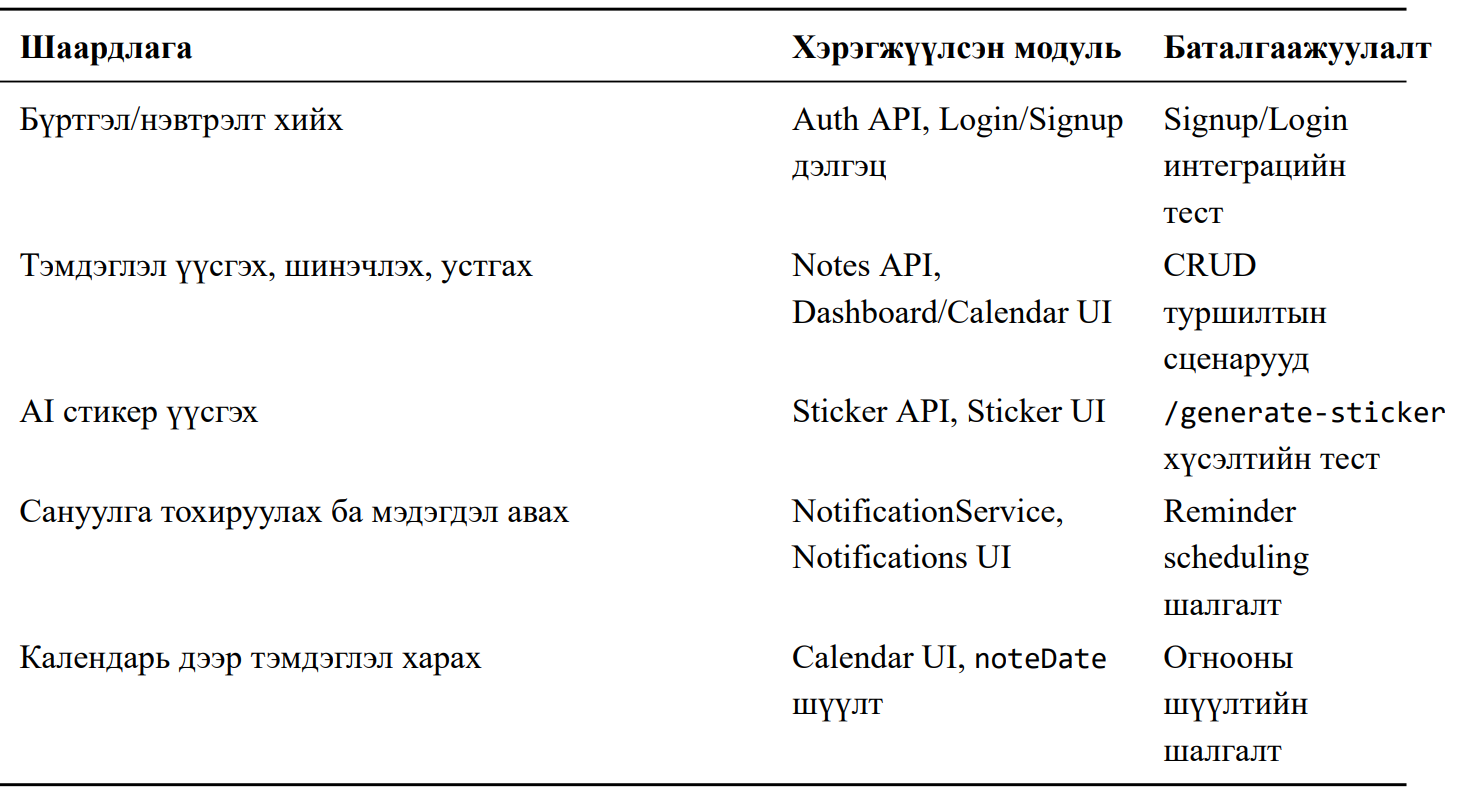
\includegraphics[width=\columnwidth]{Pictures/11.png}

Мөн өгөгдлийн урсгалыг контекст түвшнээс
эхлэн шаталсан (DFD level 0--2) байдлаар
задлан тайлбарлаж, хэрэглэгчийн үйлдлээс
эхлээд өгөгдлийн сан болон хиймэл оюуны
үйлчилгээ хүртэлх урсгалыг тодорхойлсон.
Доор контекст түвшин болон нэгдүгээр
түвшинийг харуулав.

\vspace{0.2cm}
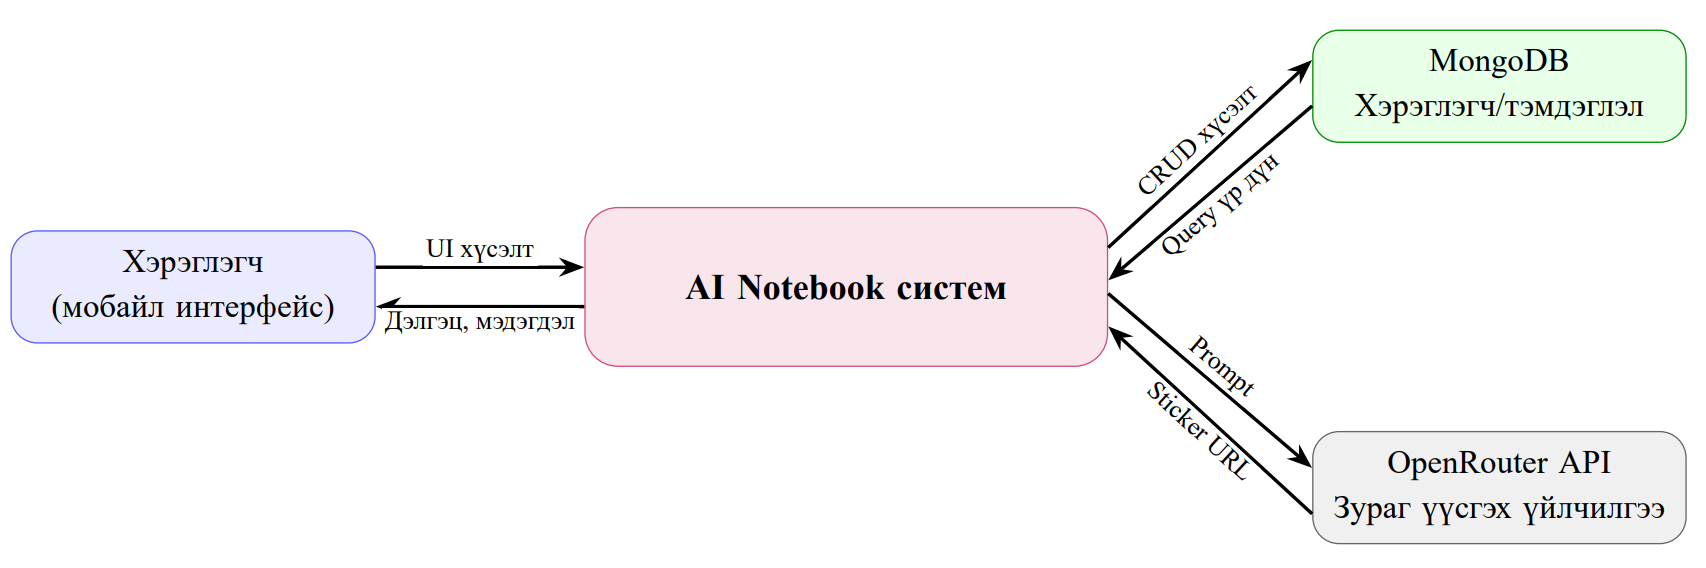
\includegraphics[width=\columnwidth]{Pictures/12.png}
\begin{flushright}
\textit{\small Зураг 2.1 Контекст түвшний өгөгдлийн урсгалын зураг}
\end{flushright}

\vspace{0.2cm}
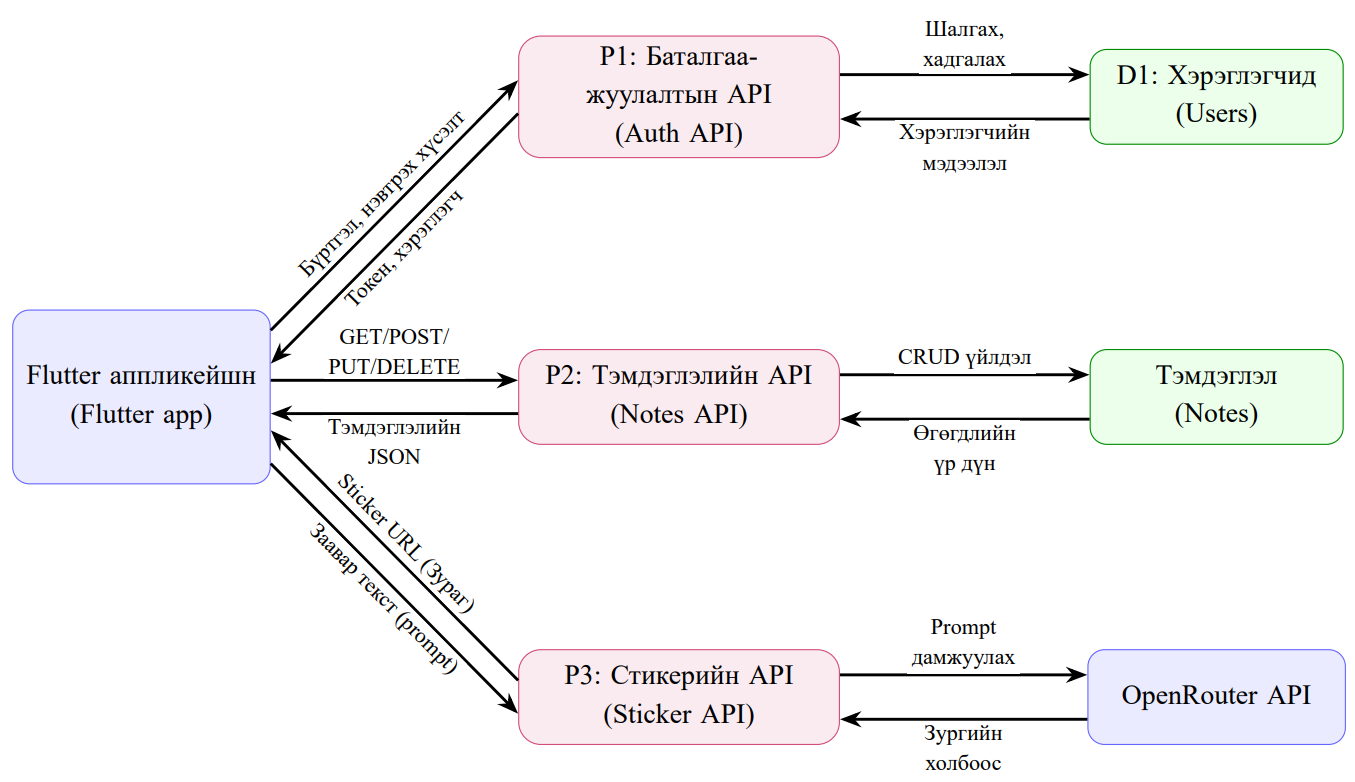
\includegraphics[width=\columnwidth]{Pictures/13.png}
\begin{flushright}
\textit{\small Зураг 2.2 Нэгдүгээр түвшний өгөгдлийн урсгал: сервер талын
модулийн задаргаа}
\end{flushright}

\textbf{3. Судалгааны үр дүн}

Системийн интеграцийн түвшинд гол
урсгалууд амжилттай баталгаажсан.

\vspace{0.2cm}
\begin{flushright}
\textit{\small Хүснэгт 3.1 Интеграцийн туршилтын үр дүнгийн нэгтгэл}
\end{flushright}
\vspace{-0.2cm}
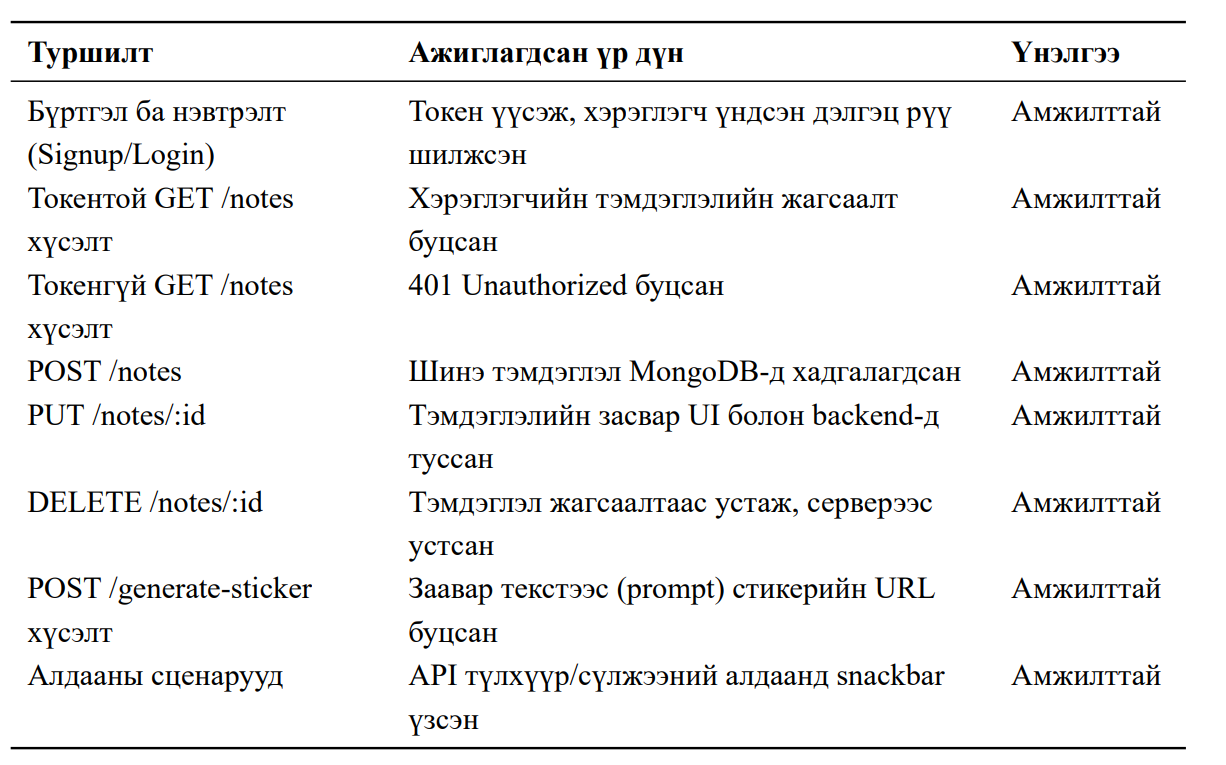
\includegraphics[width=\columnwidth]{Pictures/14.png}

Стикер үүсгэх урсгалд дараах үе шат
баталгаажсан:

\begin{itemize}
\item Клиент талаас POST
/api/notes/generate‐sticker хүсэлтээр prompt
илгээнэ;
\item Backend OpenRouter API руу хүсэлт
дамжуулж зураг үүсгэнэ (model: flux-pro
эсвэл fallback);
\item URL эсвэл алдааны хариу буцаана;
\item Frontend сүүлийн тэмдэглэлийн stickerUrl
талбарт хадгалж, preview харуулна.
\end{itemize}

Гүйцэтгэлийн бодит хэмжилт
S1, S2, S3 туршилтын сценаруудыг бодит
backend орчинд ажиллуулж,
/api/notes/generate‐sticker төгсгөлийн цэгийн
latency болон CPU ачааллыг хэмжив.

\vspace{0.2cm}
\begin{flushright}
\textit{\small Хүснэгт 3.2 Generative AI туршилтын бодит хэмжилтийн үр дүн}
\end{flushright}
\vspace{-0.2cm}
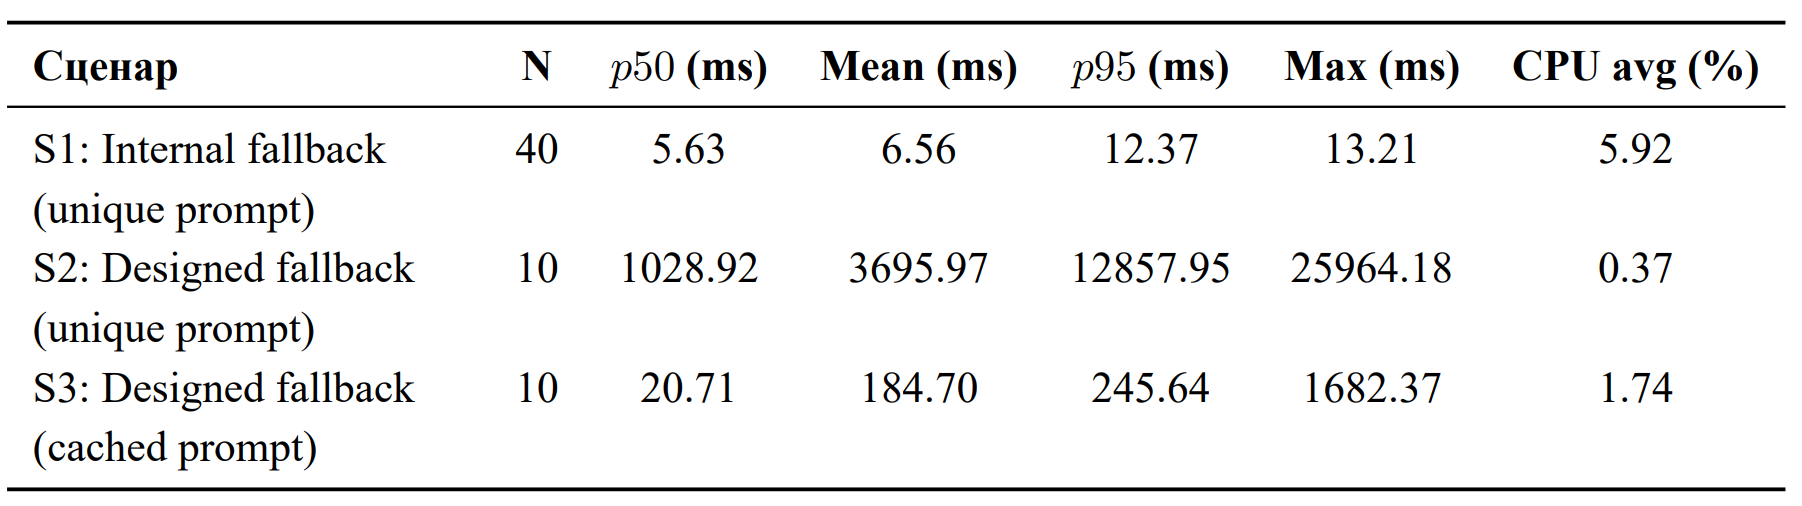
\includegraphics[width=\columnwidth]{Pictures/21.png}

\textbf{4. Дүгнэлт}

Энэхүү судалгааны ажлаар гар утасны
хэрэглээний харагдах хэсэг, сервер талын
хэсэг, өгөгдлийн сан болон хиймэл оюуны
үйлчилгээний нэгтгэлийг ашиглан ``AI
Notebook'' системийг бодит түвшинд
хэрэгжүүлж, тэмдэглэл үүсгэх, унших,
шинэчлэх, устгах үйлдэл болон хиймэл оюун
ухаанаар стикер үүсгэх үндсэн боломжуудыг
нэгтгэн амжилттай туршиж нотолсон.
Судалгааны үр дүнгээс үзэхэд
модульчлагдсан бүтэц, токенд суурилсан
хамгаалалт, өгөгдлийн урсгал болон
дарааллын диаграммын уялдаа холбоо нь
системийн ажиллагааг ойлгомжтой, өргөтгөх
болон хэрэглээнд нэвтрүүлэх боломжтой
шийдэл гэж дүгнэж байна.

\textbf{5. Ном зүй}

[1] Google. Flutter documentation.
https://docs.flutter.dev, 2026.

[2] OpenJS Foundation. Node.js documentation.
https://nodejs.org/en/docs, 2026.

[3] MongoDB Inc. MongoDB manual.

https://www.mongodb.com/docs/manual, 2026.

[4] Michael Jones, John Bradley, and Nat Sakimura.
RFC 7519: JSON Web Token (JWT).
https://www.rfc-editor.org/rfc/rfc7519, 2015.

\end{multicols}




\clearpage
\pagenumbering{arabic}
\setcounter{page}{1}

\addtotoc{Abstract}
\thispagestyle{plain}


\begin{center}
{\Large\bfseries DEVELOPMENT OF A DIGITAL NOTEBOOK APPLICATION}
\end{center}

\begin{flushright}
\small
DEPARTMENT OF COMPUTER SCIENCE

Student: s21c032b, E. Anu\\
Supervisor: U. Anujin
\end{flushright}

\setlength{\columnsep}{5mm}
\setlength{\parindent}{0pt}

\begin{multicols}{2}

\small

\textbf{1. Introduction}

In modern times, people have an increasing need to regularly record their daily tasks, studies,
and personal plans. However, paper-based notes can be easily lost, are inconvenient to carry,
and make information retrieval difficult. At the same time, many existing note-taking applications
have limited reminder and additional features. Therefore, there is a need for an intelligent digital
note-taking solution that can generate stickers, provide reminders, and include a calendar view.

Based on this requirement, this work developed and implemented the “AI Notebook” system.

\textbf{Goal}

The main goal of this research is to design, develop, and evaluate a mobile application for intelligent
note-taking based on frontend and backend architecture, including user authentication, note management,
and AI-based sticker generation.

\textbf{2. Research Methodology}

This research applied the Design Science Research methodology, which includes iterative phases of
requirement analysis, architecture design, system development, testing, and validation.

At the methodological level:
\begin{itemize}
\item Data Flow Diagrams (DFD) were developed at context, level 1, and level 2 to describe system flows.
\item Sequence diagrams were used to model login, note creation, sticker generation, and notification workflows.
\item Integration testing was performed, including API flow testing, token authentication, error handling,
and performance measurement.
\end{itemize}

Functional and non-functional requirements were defined separately, and a traceability matrix was used
to show how each requirement is implemented and verified across modules.

\vspace{0.2cm}
\begin{flushright}
\textit{\small Table 2.1 Functional Requirements Traceability Matrix}
\end{flushright}
\vspace{-0.2cm}
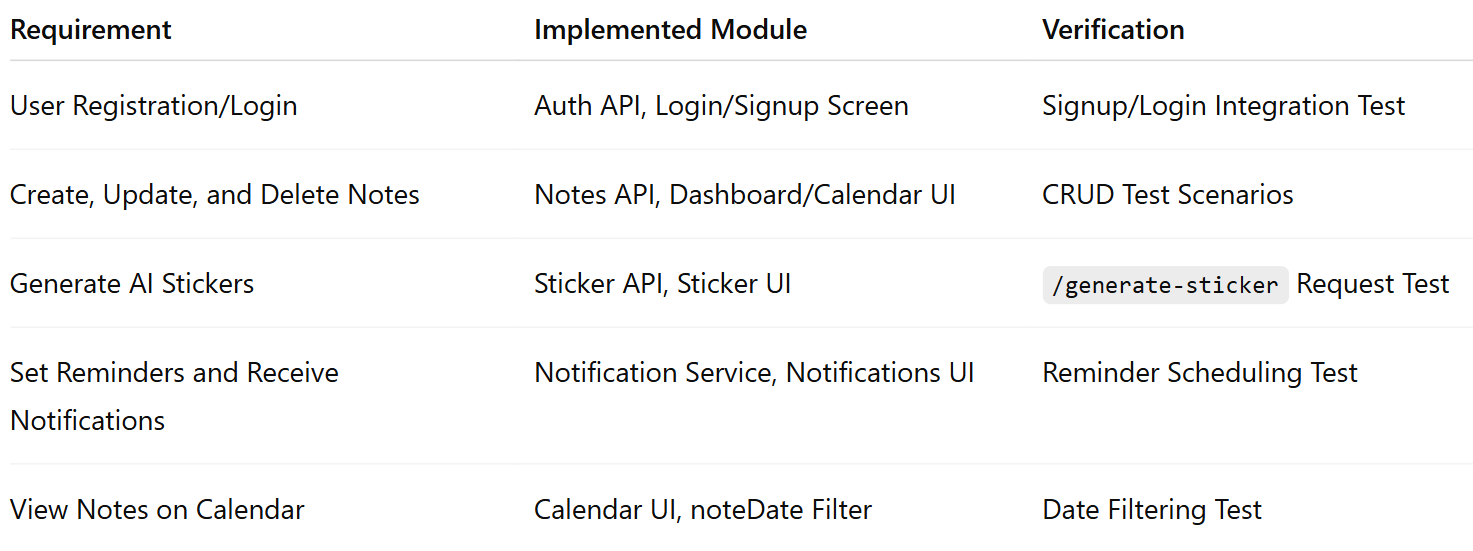
\includegraphics[width=\columnwidth]{Pictures/11.1.png}

In addition, data flows were analyzed from context level down to hierarchical levels (DFD level 0–2),
covering the flow from user actions to database and AI services. The context and level 1 diagrams are
shown below.

\vspace{0.2cm}
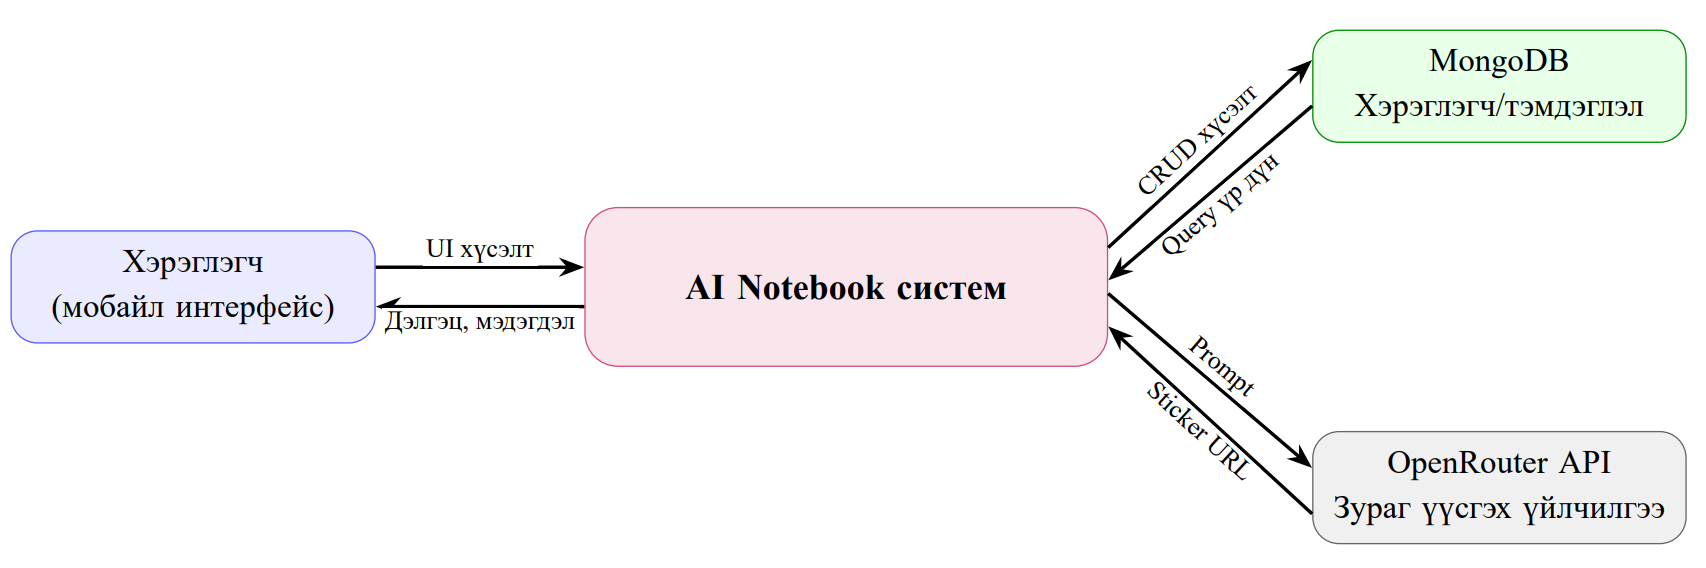
\includegraphics[width=\columnwidth]{Pictures/12.png}
\begin{flushright}
\textit{\small Figure 2.1 Context-Level Data Flow Diagram}
\end{flushright}

\vspace{0.2cm}
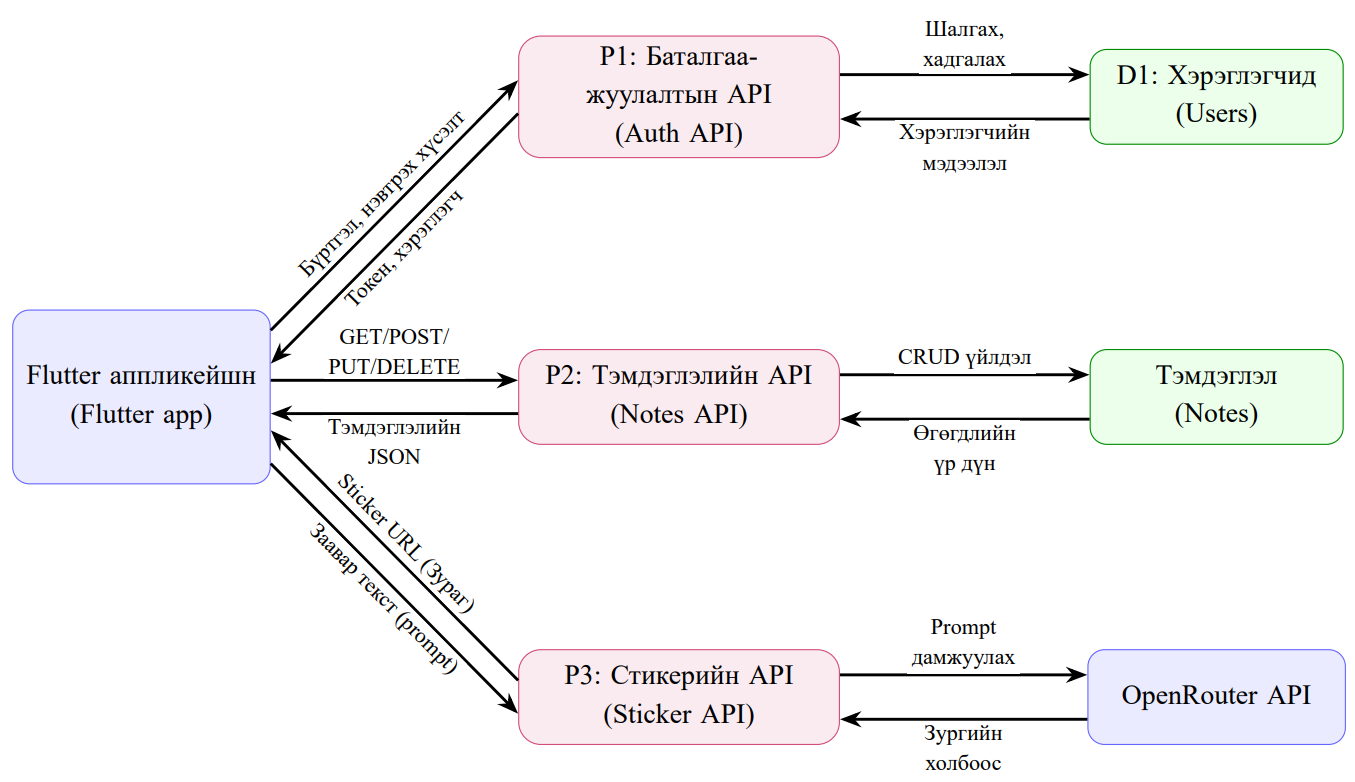
\includegraphics[width=\columnwidth]{Pictures/13.png}
\begin{flushright}
\textit{\small Figure 2.2 Level 1 Data Flow Diagram: Backend Module Decomposition}
\end{flushright}

\textbf{3. Results}

At the system integration level, the main workflows were successfully validated.

\vspace{0.2cm}
\begin{flushright}
\textit{\small Table 3.1 Summary of Integration Testing Results}
\end{flushright}
\vspace{-0.2cm}
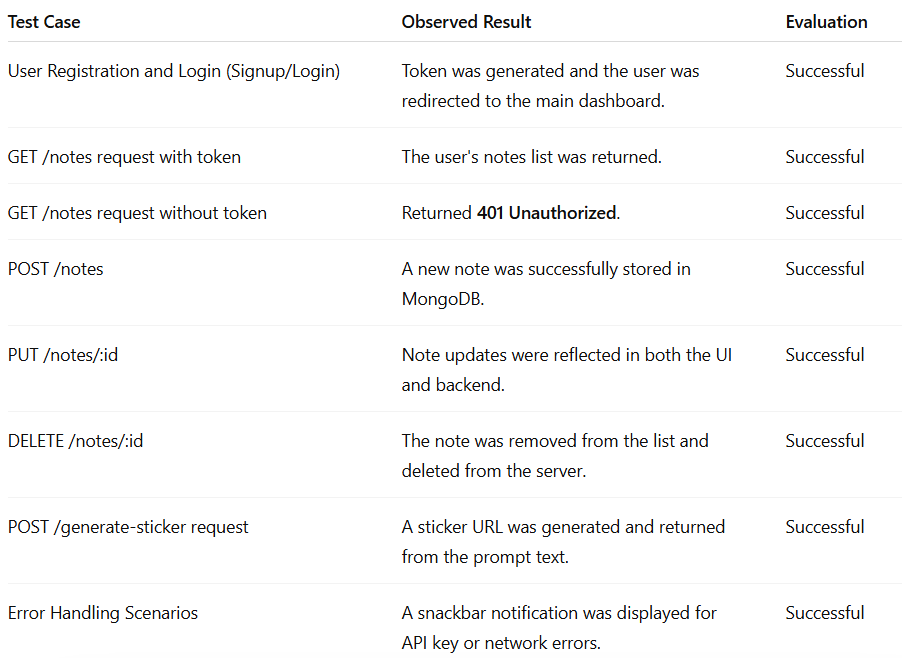
\includegraphics[width=\columnwidth]{Pictures/14.1.png}

The following steps were confirmed in the sticker generation workflow:

\begin{itemize}
\item The client sends a POST request to /api/notes/generate-sticker with a prompt;
\item The backend forwards the request to the OpenRouter API to generate an image (model: flux-pro or fallback);
\item A URL or error response is returned;
\item The frontend stores the stickerUrl in the latest note and displays a preview.
\end{itemize}

Performance measurements were conducted using real backend environments with S1, S2, and S3 test scenarios,
measuring latency and CPU load of the /api/notes/generate-sticker endpoint.

\vspace{0.2cm}
\begin{flushright}
\textit{\small Table 3.2 Real Performance Results of Generative AI Testing}
\end{flushright}
\vspace{-0.2cm}
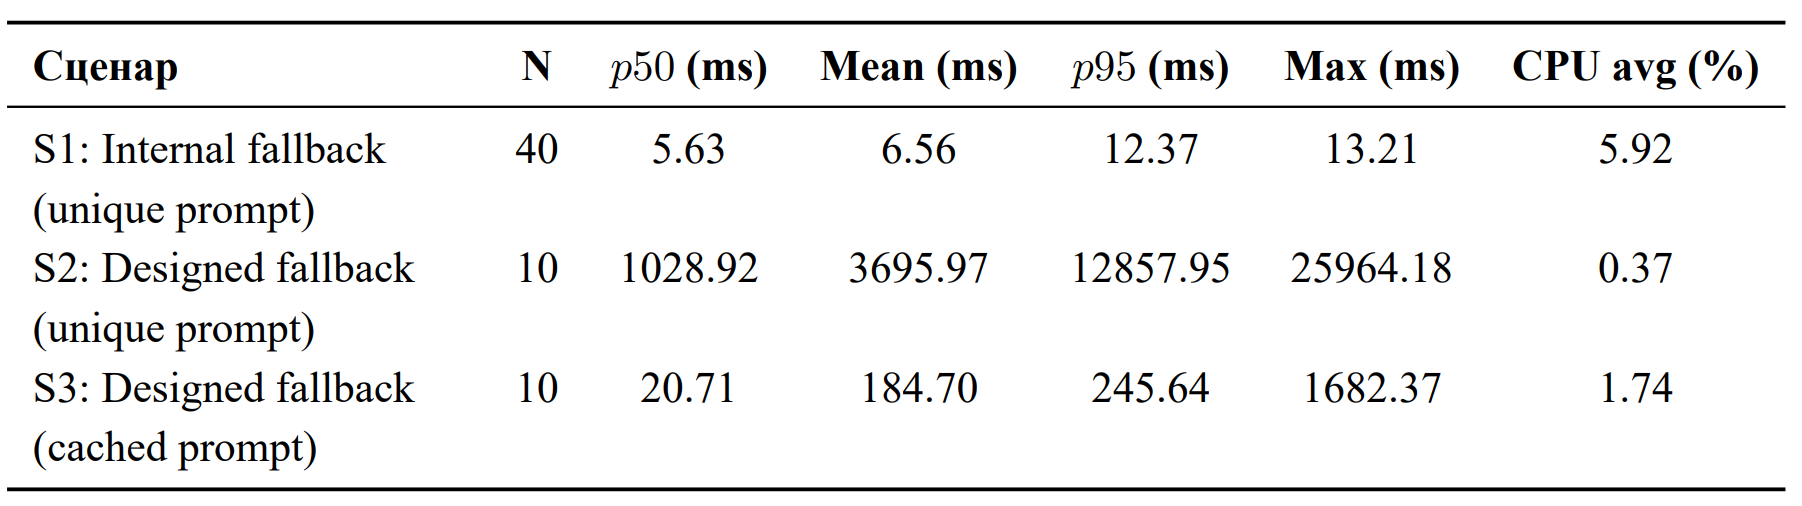
\includegraphics[width=\columnwidth]{Pictures/21.png}

\textbf{4. Conclusion}

This research successfully implemented an “AI Notebook” system by integrating mobile frontend,
backend services, database, and artificial intelligence components. The system supports core features
such as creating, reading, updating, and deleting notes, as well as AI-based sticker generation.

The results show that a modular architecture, token-based authentication, data flow design,
and sequence modeling contribute to a system that is understandable, scalable, and suitable for real-world deployment.

\textbf{5. References}

[1] Google. Flutter documentation.
https://docs.flutter.dev, 2026.

[2] OpenJS Foundation. Node.js documentation.
https://nodejs.org/en/docs, 2026.

[3] MongoDB Inc. MongoDB manual.

https://www.mongodb.com/docs/manual, 2026.

[4] Michael Jones, John Bradley, and Nat Sakimura.
RFC 7519: JSON Web Token (JWT).
https://www.rfc-editor.org/rfc/rfc7519, 2015.

\end{multicols}

\end{document}
